\documentclass[12pt, a4paper]{memoir} % for a short document
\usepackage[french,english]{babel}

\usepackage [vscale=0.76,includehead]{geometry}                % See geometry.pdf to learn the layout options. There are lots.
%\geometry{a4paper}                   % ... or a4paper or a5paper or ... 
%\geometry{landscape}                % Activate for for rotated page geometry
%\OnehalfSpacing
% \setSingleSpace{1.05}
%\usepackage[parfill]{parskip}    % Activate to begin paragraphs with an empty line rather than an indent
\usepackage{graphicx}
\usepackage{amsmath}
\usepackage{fullpage}
\usepackage{mathptmx} % font = times
\usepackage{helvet} % font sf = helvetica
\usepackage[latin1]{inputenc}
\usepackage{relsize}
\usepackage{verbatim} 

%Style des ttes de section, headings, chapitre
\headstyles{komalike}
\nouppercaseheads
\chapterstyle{dash}
\makeevenhead{headings}{\sffamily\thepage}{}{\sffamily\leftmark} 
\makeoddhead{headings}{\sffamily\rightmark}{}{\sffamily\thepage}
\makeoddfoot{plain}{}{}{} % Pages chapitre. 
\makeheadrule{headings}{\textwidth}{\normalrulethickness}
%\renewcommand{\leftmark}{\thechapter ---}
\renewcommand{\chaptername}{\relax}
\renewcommand{\chaptitlefont}{ \sffamily\bfseries \LARGE}
\renewcommand{\chapnumfont}{ \sffamily\bfseries \LARGE}
\setsecnumdepth{subsection}


% Title page formatting -- do not change!
\pretitle{\HUGE\sffamily \bfseries\begin{center}} 
\posttitle{\end{center}}
\preauthor{\LARGE  \sffamily \bfseries\begin{center}}
\postauthor{\par\end{center}}

\newcommand{\jury}[1]{% 
\gdef\juryB{#1}} 
\newcommand{\juryB}{} 
\newcommand{\session}[1]{% 
\gdef\sessionB{#1}} 
\newcommand{\sessionB}{} 
\newcommand{\option}[1]{% 
\gdef\optionB{#1}} 
\newcommand{\optionB}{} 

\renewcommand{\maketitlehookd}{% 
\vfill{}  \large\par\noindent  
\begin{center}\juryB \bigskip\sessionB\end{center}
\vspace{-1.5cm}}
\renewcommand{\maketitlehooka}{% 
\vspace{-1.5cm}\noindent
\includegraphics[height=14ex]{img/logoINP.png}\hfill\raisebox{2ex}{
\includegraphics[height=7ex]{img/logoUJF.jpg}}\\
\bigskip
\begin{center} \large
Master of Science in Informatics at Grenoble \\
Master Math\'ematiques Informatique - sp\'ecialit\'e Informatique \\ 
option \optionB  \end{center}\vfill}
% End of title page formatting

\option{PDES}
\title{Efficient dynamic and static environment classification in Occupancy Grid framework}%\\\vspace{-1ex}\rule{10ex}{0.5pt} \\sub-title} 
\author{Botelho do Nascimento, Jander}
\date{ $<$Defense Date$>$} % Delete this line to display the current date
\jury{
Research project performed at Inria \\\medskip
Under the supervision of:\\
Qadeer Baig (\texttt{qadeer.baig@inria.fr}), Inria \\
Mathias Perrollaz (\texttt{mathias.perrollaz@inria.fr}), Inria \\\medskip
Defended before a jury composed of:\\
$[$Prof/Dr/Mrs/Mr$]$ $<$first-name last-name$>$\\
$[$Prof/Dr/Mrs/Mr$]$ $<$first-name last-name$>$\\
$[$Prof/Dr/Mrs/Mr$]$ $<$first-name last-name$>$\\
$[$Prof/Dr/Mrs/Mr$]$ $<$first-name last-name$>$\\
}
\session{$[$June/September$]$\hfill year}


%%% BEGIN DOCUMENT
\begin{document}
\selectlanguage{english} % french si rapport en franais
\frontmatter
\begin{titlingpage}
\maketitle
\end{titlingpage}

%\small
\setlength{\parskip}{-1pt plus 1pt}

\renewcommand{\abstracttextfont}{\normalfont}
\abstractintoc
\begin{abstract} 
Scene understanding is a fundamental process in robotics. Several techniques have been applied with the intent to better classify the objects in the scene with more quality and/or a better performance. The occupancy grid is refereed by many as one of the major tools to represent the environment, gathering precision and performance in the representation. The algorithm proposed by this document extracts the dynamic objects from the environment with the smallest possible number of samples using occupancy grid mapping, resulting in a lightweight real-time application. The main focus is to apply it, in the future, for  Advanced Driving Assistence Systems(ADAS). Throughout this document we will show some issues imposed by the usage of our algorithm in ADAS, and solution for those problems. Qualitative results of the algorithm implementation in a Lexus LS600h car for the real road application will be shown, followed by a discussion about the advantages and limitations of the method.

%\end{abstract}
%\abstractintoc
%\renewcommand\abstractname{R\'esum\'e}
%\begin{abstract} \selectlanguage{french}
%Texte 
%\end{abstract}
%\selectlanguage{english}% french si rapport en franais


\end{abstract}
%\abstractintoc
%\renewcommand\abstractname{R\'esum\'e}
%\begin{abstract} \selectlanguage{french}
%Texte 
%\end{abstract}
%\selectlanguage{english}% french si rapport en franais

\cleardoublepage

\tableofcontents* 

\normalsize

\mainmatter
\SingleSpace

\chapter{Introduction} 
	\section{Driving support systems}

In this document we are mainly concerned about driving assistance systems. Such system facilitates the task of driving. This support can appear in several forms: 

\begin{itemize}
\item visual alerts
\item auditory alerts
\item tactile alerts (also known as haptics\cite{riener2010sensor})
\end{itemize}

Driving support system may also provide support in a less passive manner as well:

\begin{itemize}
\item change how the car respond to the drivers commands for assisting a maneuver
\item change how the car behaves, with partial or fully automatic command
\end{itemize}

This field has gained several adepts. Automotive industry and researchers are studying it thoroughly these days.

Thus, driving support systems and its applications are becoming a popular tool. To exemplify such change, some countries changed their laws to make mandatory that all new cars manufactured have a given support system installed as a minimum equipment, ABS(Anti-lock break systems)  for instance \footnote{http://www.estadao.com.br/noticias/impresso,freio-abs-passa-a-ser-obrigatorio,351726,0.htm}.

One of the reasons for such change is the increasing number of incidents involving vehicles. \textbf{Risk of incidents} is growing as the population of cars grows, and there is no signal in changing those numbers in next years, so driving support systems is coping with task of making the car a safer transportation system, among others tasks (Figure~\ref{fig:sensor:target}).

Those incidents may be related with the cognitive capacity limitation of the human being. With the goal of quantify this capacity, a research conducted in 2008 studied the human cognitive limitation for visual sensing mechanism \cite{LautarutisV}. This report established the limit number of objects which the human is capable of track simultaneously. This study establishes the limit of the human vision by associating it with the information channel capacity theorem (Shannon's theorem). 

Although this seems to be distant from our goal (safety), this research underlies the limitation of human driving skills. With it we can conclude that above certain number of surrounding vehicles, we may start to ignore the risk of collision with some vehicles that still may represent a risk. Besides, several factors can affect its behavior like fatigue, cognitive capacity or simply bad decisions.

%Although, cognition is not an absolute number it varies according to several parameters, like mental health, type of sensing mechanism (visual, auditory, tactile), amount of information transmitted, etc. 

The action of driving did not change considerably since its creation but several mechanisms to support the driver have been included in the vehicle. All to provide a comfortable and safer experience for the driver\cite{riener2010sensor}.

A more modern approach of driving support system has appeared: Advanced Driver Assistance Systems (ADAS). 

ADAS relies in computerized systems to process informations provided by the car (through sensors) to improve the user experience. 

ADAS is split in different research branches, each of them with its own applications and goals. Among those different branches (Figure \ref{fig:sensor:target}), our work will concentrate in supporting applications situated in \textbf{safety} branch. 

The goal of this work is to tackle a very common issue in safety application (object classification) and \textbf{not} develop an application.

This will be done by providing a theoretical framework to classify the environment in a high level manner, separating static and dynamic parts with the information acquired from the sensors.

\begin{figure}[h]
\centering
	\begin{tabular}{lr}\\
		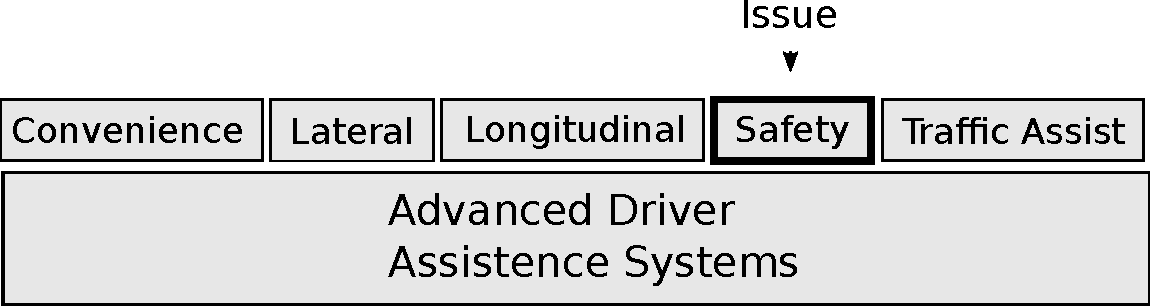
\includegraphics[scale=0.7]{img/fig:sensor:target} 
	\end{tabular}
	\caption{ADAS application stack and problem to be tacked (adapted from \cite{riener2010sensor})}
	\label{fig:sensor:target}
\end{figure}

Advanced Driver Assistance Systems rely on the perception. An ADAS works somehow similar to the human cognition, it requires a mean to perceive the environment before dispatch any action. 

There are different ways of perceiving the environment, usually we observe specific features, like: lighting, appearance, shapes, etc. Every feature requires a mechanism to process the information and convert the physical characteristics into electronic signal. The peripherals responsible for this process are called sensors, which will be discussed in more details in the Section \ref{sec:sensors}.

%% reviewed until here

\subsection{Sensors}
\label{sec:sensors}

%maybe replace the world system in the diagram and text by "control systems"

Sensing is the input for numerous biological systems (\textit{e.g.} nervous system, digestive system), enabling such systems to respond properly to the information provided by such sensors(eye, skin, etc.). 

This scheme is as important to robotics as they are for human being. In order to interact with the environment, a robot needs first to perceive it. This is done by capturing specific features, or at least some of them. The features observed depends on the application needs.

\begin{figure}[h]
   \centering
     \begin{tabular}{lr}
       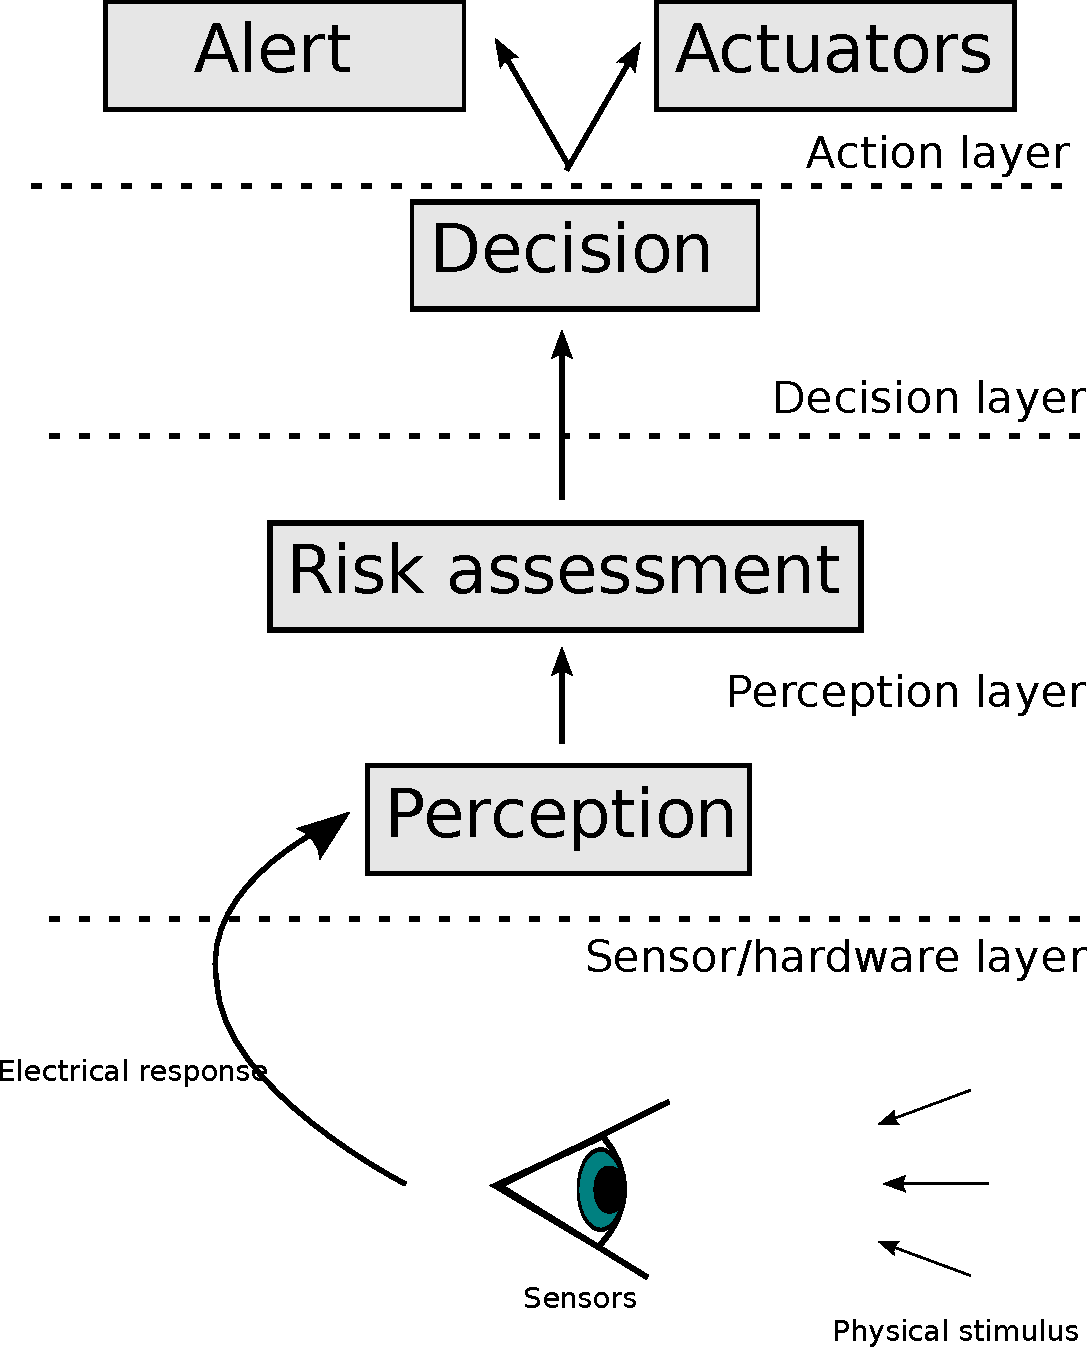
\includegraphics[scale=0.45]{img/fig:sensors:roles}
     \end{tabular}
   \caption{A general architecture of a system attached to sensors}
   \label{fig:sensors:role}
 \end{figure}

Sensors are the means in which complex systems acquire information about the environment. Although, the sensors play a key role in almost every systems. It is not their role to process information, only acquire them (Figure \ref{fig:sensors:role}). 

The sensors are normally incapable to respond to external stimulus without a system to process the data provided by it, and act. The system reacts to the sensor stimulus through other means.

Thus, a sensor is responsible for the data acquisition (electric interpretation of a physical stimulus). This data is directed to a perception layer which is allocated in an upper layer, which is responsible for the understanding of the environment and the objects located in it. 

In the \textit{risk assessment layer} is where the decisions are taken, this turns it into the main layer for the actual result of the safety application.

\subsubsection{Types}

There are virtually sensors for all kinds of properties (Figure~\ref{fig:sensors}) that we want to observe. In some literatures those properties can be called \textbf{measurands}\cite{riener2010sensor}. 

There exists two sets of classifications for sensors, they can be Proprioceptive/Exteroceptive with respect to the type of measurands \cite{iyengar1991autonomous} and they are classified in the manner how the measurands are obtained, which can be in a passive or active \cite{Hebert_2000_3595} manner. Active sensors emit energy to the environment so the measurand can be collected, a passive sensor is capable of observing the measurand without emit any type of energy in the environment.

Active and passive type refer to the electronic means in which the measurand is obtained. A second sensor typing is defined according to the target subject of the measurand, they can be proprioceptive and exteroceptive.

\textit{Proprioceptive} evaluate the ego-robot properties, giving informations about some \textbf{measurand} of the robot itself. Motor speed, payload, robot joint angles, battery voltage are some examples.  Inertial Measurement Unit (IMU) is a \textit{proprioceptive} sensor that observes the orientation, velocity and gravitational forces of the robot, it is a very common type of sensor and largely applied in robotics and in aviation.

\textit{Exteroceptive} gives information about the environment in which the robot is located. Thus, they extract useful environmental features. Light intensity and sound amplitude are some examples of \textit{exteroceptive} sensor.

\begin{figure}[h]
   \centering
     \begin{tabular}{lr}
       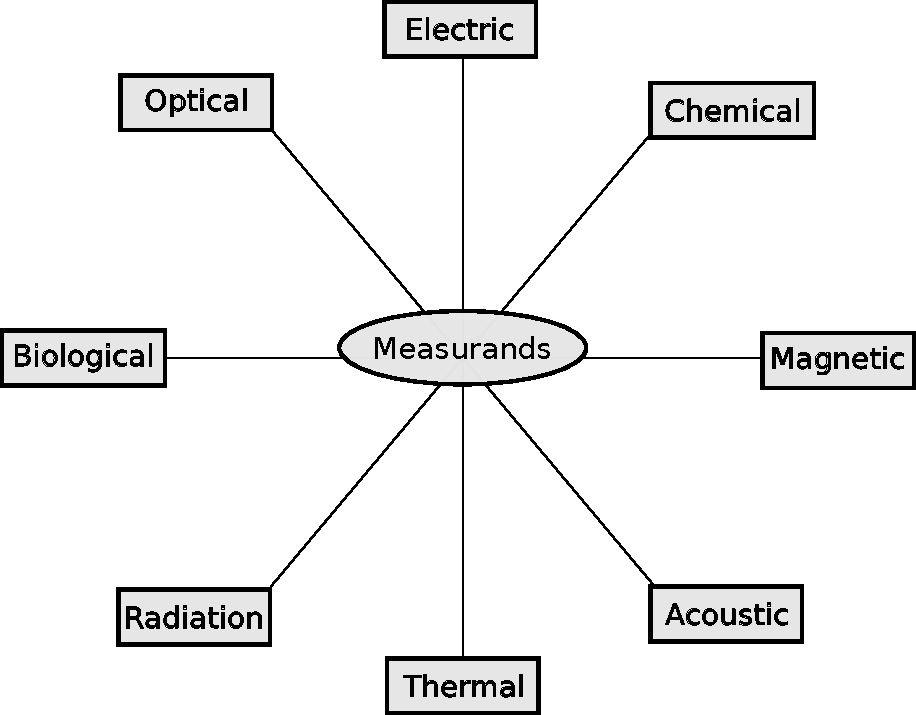
\includegraphics[scale=0.70]{img/fig:sensors}
     \end{tabular}
   \caption{Different types of measurands (adapted from \cite{WhiteRichard})}
   \label{fig:sensors}
 \end{figure}

\subsubsection{Properties}

The sensors are subject to issues. As the sensor is the capacity of a system to observe the environment, this affects directly any subsequent processing.

The most common issues are: imprecision, uncertainty and incomplete data. 

\paragraph{Imprecision} Sensors rely on physical properties of the observed \textbf{measurands}, those properties may vary according to the environment in which the sensor is deployed.

Laser scanner can be an example of sensor with imprecision. Laser scanner uses light to measure the distance from objects, it does this by counting the time taken to the light to hit an object and be reflected back called Time-of-Flight(ToF). Although in absence of oxygen the speed of the light is constant, on earth it depends on density of the atmosphere, amount of water particles in the air, among others chemical elements. The presence of those elements change the speed of the light, and as the presence of each individual component may vary according to the geographic region the result of ToF varies accordingly. Thus, influencing the sensor measurements.

\paragraph{Incomplete data} Due to the limited capacity of the sensors to capture the details of the environment, the data provided by them can be incomplete, by meaning that certain regions of the environment are not reachable and nothing can be said about that specific region. As example we can take the laser scanners, they measure the distance between the sensor and an intercepting object. In this situation, nothing can be said beyond the intercepting object. Thus it is an incomplete data.

\subsection{Risk assessment}
\label{sec:riskassessment}

\textbf{Risk Assessment} is a term adopted in several fields to indicate the mitigation of the consequences involved in a target activity. 

Before describe Risk Assessment and its relation with ADAS we first must understand what risk means. Mainly how we are going to apply this concept in this document. 

\textbf{Risk} is anything that can affect (negatively or positively) a subject \cite{mulcahy2011pmp}. By positive meaning that if a situation $A$ happens to be true something good may happen in the future to the target subject, or negative meaning if situation $B$ happens to be true, the subject may suffer negative consequences in the future. It is a common practice to track just the negative risks, that is why positive risk looks so unfamiliar for most of the readers. 

Some literature use another terms to indicate negative risk, like hazard or threat. In this document we are going to apply the term \textit{risk} mainly. It will gain the negative risk meaning.

\textit{Risk assessment} is the action of studying what variations can cause risk the subject, the origin of the cause can be \textbf{direct} or \textbf{indirect}.

A didactic example to illustrate the \textbf{direct} and \textbf{indirect} situations: imagine you bought a very good amount of shares from Apple Inc\copyright. But you forgot that its products are manufactured in an Asian country. Suddenly this Asian country government announces that it is forbidden to export any kind of product to western countries. 

Well, needless to say that you are bankrupt. Something that was not directly related - international diplomacy relations - to your subject can affect dramatically its value. We can refer to the subject as assets, or future assets.

Thus, the subject can be anything with enough degree of importance to justify the risk assessment. Some examples are: a project, stock market share, a schedule, an action.

Risk assessment applied in ADAS is generally done to evaluate the risk of collision between vehicles. Thus, we are worried about direct risk. 

This is done by perceiving the environment, specifically the dynamic environment. The dynamic environment is chosen to be studied rather than static due to its close relationship with  collisions situations. 

The collisions can be caused by several factors, but commonly other vehicles sharing the same space are responsible for a big part of the collisions, the study \cite{Hurt_1981} showed statistically that $75\%$ of collisions are between two vehicles, and only $22\%$ are vehicles in collision with other objects. Therefore, the relationship among dynamic objects are important for the risk assessment.

\section{Perception}

Before talking about perception, it is necessary to comprehend few concepts. Those concepts will frequently appear during this work: \textit{localization}, \textit{mapping}, \textit{tracking}, \textit{detection} and \textit{classification}.

All those terms are largely applied in robotics and they correspond to actions that supports the interpretation of  the environment or the elements in it.

\textbf{Localization} provides the coordinates of a point with respect to a another point, known as frame reference. If this frame of reference is the earth, for instance, we call it global frame of reference. In robotics, depending on the application of the robot we can have different frames of reference. We can use a building as frame of reference, by indicating the position of the robot with respect to this building (having a point of the building as the origin). The robot's position may be given in a global reference of frame, meaning that wherever the robot is located in the earth globe, we can provide a coordinate to represent its position. 

The result of \textbf{mapping}, as tacit knowledge, is a processing that gives us information about a region, a limited area. Allowing to give a more concrete definition by being the action of recording the disposition of the static objects of a region. The data recorded can be used later in the future as a fundamental information for exploration purpose. In a geological map for instance the static objects are rivers, mountains, canyons, etc. 

\textbf{Localization and Mapping} are really important tools for a robot, due to their importance and relation the term SLAM was coined to represent those two tasks (more details in next chapter). Although they solve part of the problem, this process is insufficient in case of existing moving objects sharing the same environment with the robot. This is due to the risk of collision between the moving objects and the robot, for this reason its necessary to detect (be aware of the existence of such object) and track (know its motion model) the object.

An easy way to understand the importance of mapping and localization, imagine the following situation: we have a map in our hands (provided by the environment \textit{mapping}) and we know exactly where we are in this map (by \textit{localization}), what would be the result of moving in this environment blind folded? Not good.

\textbf{Detection} is the action of recognize a given object in the scene, can be anything that is relevant for the scene understanding. The \textbf{tracking} consist in follow the subsequent poses assumed by the detect object during a certain amount of time. The term \textit{tracking} is usually applied with the full meaning of \textit{tracking of moving objects}\cite{Wang04a} or even \textit{moving object tracking}, but those terms can used in alternating manner in this document with exactly the same meaning.

\paragraph{The perception process} The general environment perception, represented in the Figure \ref{fig:perception:cycle}, requires at least two inputs: the perception measurements $Z$ which are usually provided by exteroceptive sensors like laser scanners, and the vehicle motion measurements $U$ that are obtained from proprioceptive sensors, like for instance an inertial measurement unit.

\begin{figure}[h]
   \centering
     \begin{tabular}{lr}
       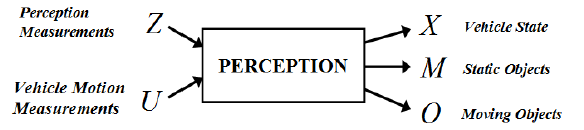
\includegraphics[scale=0.5]{img/fig:perception:cycle}
     \end{tabular}
   \caption{Perception cycle (adapted from \cite{VU-2009-454238})}
   \label{fig:perception:cycle}
 \end{figure}

In the next sections we are going to see in more details the approaches used in robotics research to tackle the localization and mapping and tracking of moving objects issues.

\subsection{SLAM}
SLAM (Simultaneous Localization and Mapping) is a process created to solve concurrently the \textit{mapping} and \textit{localization} problems\cite{VU-2009-454238}. In this approach it is assumed that the initial position of the ego-robot is unknown. 

In such process, the observation acquired by the robot's sensor must be used for estimation. The sensor readings should be enough to obtain the robot's \textit{localization}. That localization coordinates must be mapped into the current map of the environment. 

This model requires a precise \textit{mapping} of the environment. This precision is required due to parallel actions performed by the robot: moving itself in the scene (which changes the environment from the robots perspective) and localizing the robot at the same time, and as the robot motion is performed in a continuous space, any interference in the measurements are accumulated and can affect severely its localization estimation, diverging the calculated position from the real position. An Input-processing-output scheme can be seen in the Figure \ref{fig:perception:slam}.

\begin{figure}[h]
   \centering
     \begin{tabular}{lr}
       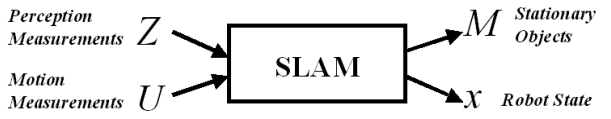
\includegraphics[scale=0.9]{img/fig:perception:slam}
     \end{tabular}
   \caption{SLAM process (adapted from \cite{Wang04a})}
   \label{fig:perception:slam}
\end{figure}

It is SLAM process responsibility to find out how to move in a certain environment having only noisy and incomplete measurements and without dynamic objects. Although, those constraints concerns just one set of application. For instance robots that are used for mining.

In the SLAM process knowing the positions that can be assumed by the robot is essential and necessary so that the robot can assume acceptable/non-occupied positions. This is done by observing the environment through the sensors and creating a spatial relationship among the static objects in this space \cite{iyengar1991autonomous}.

The robot actions are subject of physical interferences as well. It can be affected by the kind of terrain in which the robot is moving. Bringing it to the spotlight of some researchers that evaluate the slippage in direction changes at for robots that moves at high speed \cite{DBLP:conf/icra/LenainTHM11}. 

Thus, \textbf{inertial} factor plays a key role in determining how reliable the robot movements are. Other properties affects inertia such as: balance, weight distribution, grip condition, type of movement, etc. All those properties bring an imprecision factor into the movement performed by a robot. 

The output of the SLAM process is the robot state $x$ and the stationary objects map $M$, process represented in the Figure~\ref{fig:perception:slam}, captured by the \textit{perception} sensors \cite{iyengar1991autonomous}.

\subsubsection{Map representation}

Map representation is a key point to solve some of the problems related to scene understanding. Thus, the type of representation chosen can be the underline bases to achieve good results.

There exist several possible types of map that can be used to represent the robots surrounded environment. Among the alternatives for map representation, three of them gained importance, which are: \textbf{direct}, \textbf{grid} and \textbf{feature-based} \cite{Wang04a}.

\paragraph{Direct}

The direct map representation, is nothing but a straightforward representation of a sensor reading. 

This technique is frequently used in RADAR-like sensors. It depicts the point of impact of each beam (or radio wave frequency depending on the sensor) in an image. Binary image is enough to represent such images, it is easy and fast to build, can be extremely oscillating depending on the type of the sensor and the deployment depending on the quality of the sensors.

This representation uses only range measurements (\textit{e.g.} sonar, laser, etc.), this kind of representation is very convenient due to its simplicity. 

A research conducted by university of North York \cite{Lu:1997:GCR:591441.591464} focused their studies in the this issue. The fundamental problem was to obtain a local map from multiple reading, in such way that the resulting map was accurate. Those readings were done by a ego-vehicle able to move in the scenario. The scenario perceived by the robot can be seen in the Figure \ref{fig:mapping:direct:result}.

Those readings were performed by a single robot and its position was calculated based in informations provided by the IMU.

The result can be seen in the Figure \ref{fig:mapping:direct:result}. On the left image we have the original mapping, created with raw information and without any kind of filtering or preprocessing. On the right image, we have a map built with scan alignment technique\cite{Lu:1997:GCR:591441.591464}. On the second image we can see more sharp vertex and a precise alignment in the edges without mispositioned lines.

\begin{figure}[h]
\centering
	\begin{tabular}{lr}\\
		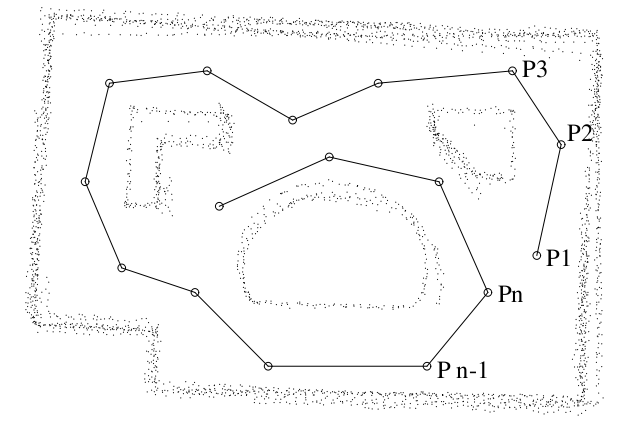
\includegraphics[width=0.5\columnwidth]{img/fig:mapping:direct:a} &
		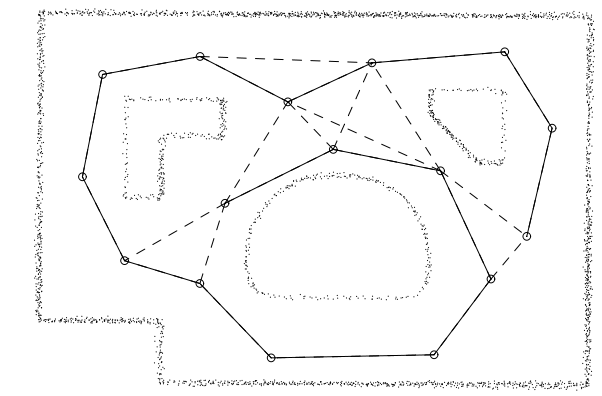
\includegraphics[width=0.5\columnwidth]{img/fig:mapping:direct:b}
	\end{tabular}
	\caption{Direct mapping result ( source \cite{Lu:1997:GCR:591441.591464} )}
	\label{fig:mapping:direct:result}
\end{figure}

Despite the good result obtained by scan alignment, it is not necessary in our approach, since we are not worried about building a map of the environment. 

\paragraph{Feature-based}

Another way to perceive the environment is the feature-based representation. In this type of map we use primitive shapes (\textit{e.g.} circles, lines, dots, ..) to represent the environment and its obstacles.

Several well known methods for detecting those features are available. Hough-transform, SIFT are good examples. 

Hough-transform is able to give us equation of lines that are part of the image. One good application for such method is to detect the edges of a road (left and right borders). By having an image of a plane road where the borders reach infinity, the Hough-transformation is capable to detect the line equation that represents the edges \cite{Ballard:1987:GHT:33517.33574}.

Scale-invariant feature transform (SIFT) detect similar points between two images, even if these similar points change in scale, noise, rotation or illumination \cite{Lowe:1999:ORL:850924.851523}.

Those methods are capable of detecting some features of an image and do a partial representation of its characteristics. 

The representation of the environment is not complete and it is subject to failures after applying the previous techniques.

This imprecise representation may generate false interpretation of the environment, that is why applying this kind of representation is not safe when ADAS is the goal platform.

\paragraph{Grid-based}
\label{ch02:gridbased}

Occupancy Grid is based on a multidimensional field that maintains the occupancy state information in a cell \cite{Elfes:1989:UOG:68491.68495}. Those cells are built in a regular size, and the number of cells which compose the grid is algorithm dependent.

By changing the size of the cells we can give more or less precision for the representation changing the resolution of the grid, which is reduce or increasing the size of the cell.

At the same time the Occupancy Grid, also known as \textit{certainty grids}, is effective in data representation it is also effective in representing sensor fusion information with it. 

Occupancy grid can be used as well to represent 3D environments, as was demonstrated in a small submersible craft, that looks for old battleships in the bottom of the ocean\cite{DBLP:journals/aim/Moravec88}.

One variation of the occupancy filter - The Bayesian Occupancy Filter(BOF) \cite{coue:inria-00182004} - contains the velocity and the probability distribution in Bayesian framework.

Representing continuous space when dealing with the uncertainty of an action of a mobile robot is extremely demanding in terms of resource usage, either in terms of processing power or memory allocation.

Thus, targeting to amortize the computational requirement for the uncertainty in the displacement of a robot, discretization models are used, Occupancy Grid\cite{Elfes:1989:UOG:68491.68495} is one of the former models proposed to tackle this issue.

This kind of representations is done with multi-dimensional vectors and results in a bird-eye view of the discretized map obtained by the perception sensor Figure \ref{fig:grid:continuous:discretized}.

\begin{figure}[h]
\centering
	\begin{tabular}{lr}\\
		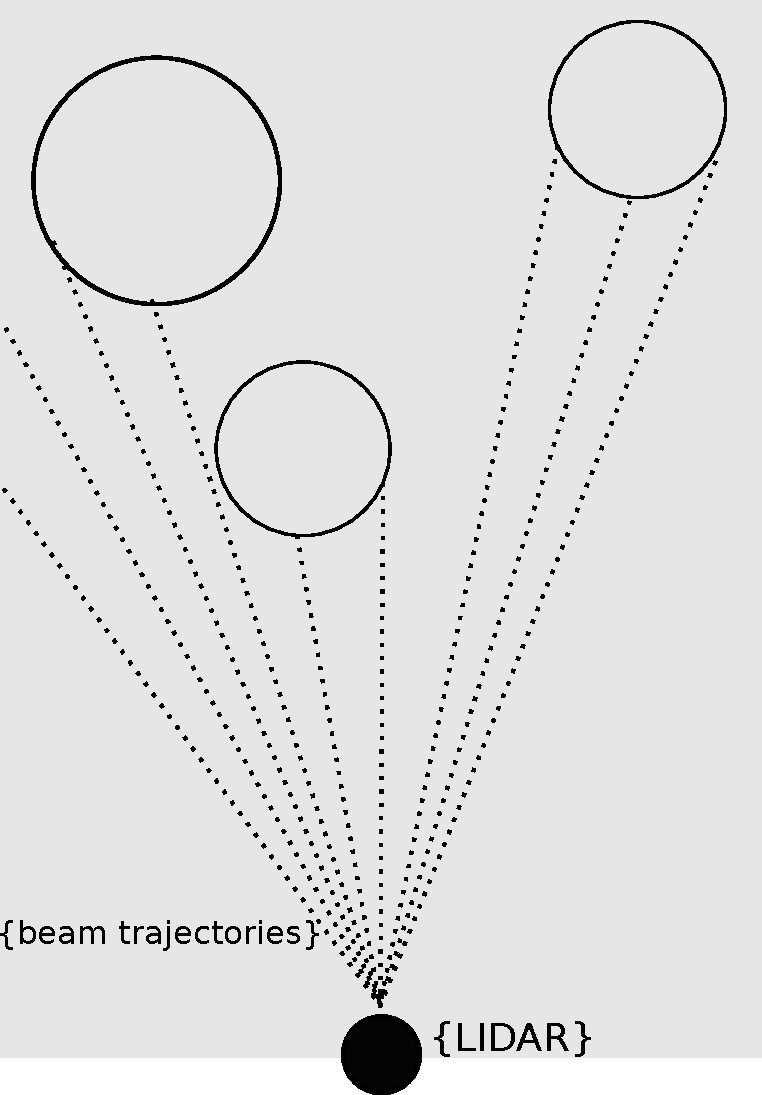
\includegraphics[width=0.25\columnwidth]{img/fig:motion:impactpoint:01} & %fig:grid:continuous
		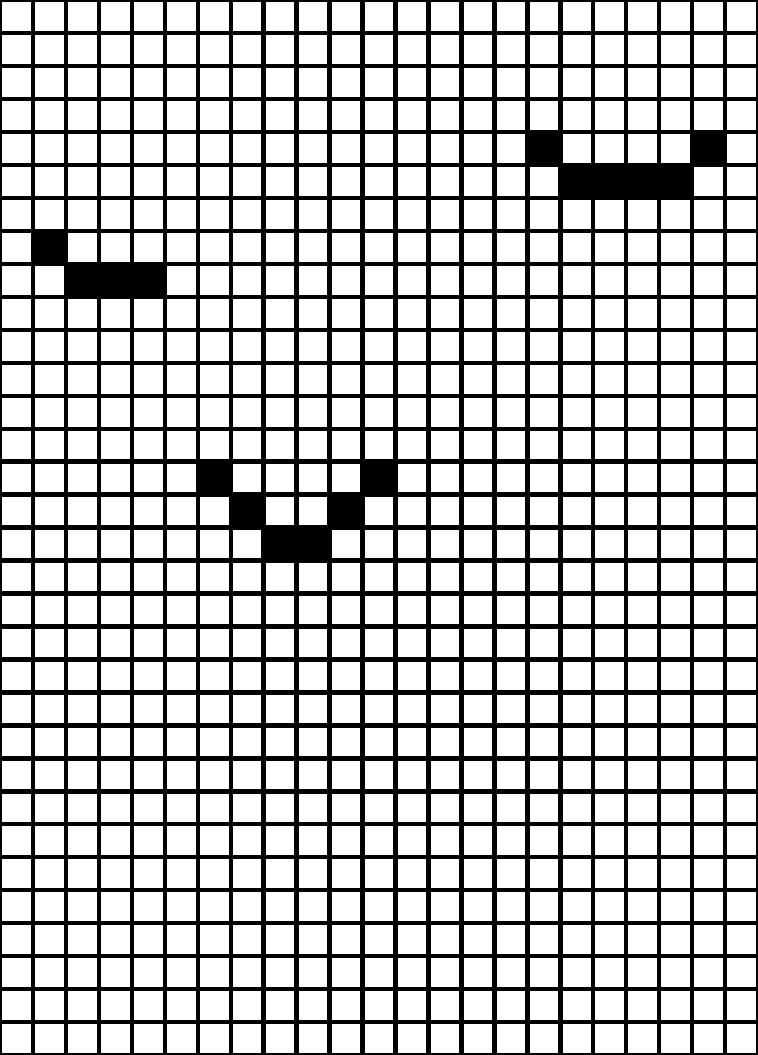
\includegraphics[width=0.25\columnwidth]{img/fig:motion:impactpoint:02} %fig:grid:discretized
	\end{tabular}
	\caption{Continuous \& discretized representation of a map}
	\label{fig:grid:continuous:discretized}
\end{figure}

In the grid framework each cell $C$ can be assigned have its state $\phi(C)$ configured to binary domain, so, either the current state of the cell is \textit{occupied} or it is \textit{free}, in this paper we state that the value $1$ represents the occupied state and $0$ a $free$ space Equation \ref{eq:binarycell}. A different domain may be used in the grid, for instance to represent random variable with a probability of occupancy of the cell (Section~\ref{sec:sensor:fusion}).

\begin{equation}
P(\phi(C)=1) + P(\phi(C)=0) = 1
\label{eq:binarycell}
\end{equation}

This model can be extended to a more general model coined as \textit{inference grids} that encapsulate multiple properties\cite{Elfes:1989:OGP:916528}.


\subsubsection{Didactic example}

In SLAM, our main concern is to localize ourselves and the static objects in the surrounding environment. 

Intending to simplify the perspective of this problem, we will generate a scenario that will be used in analogy to the formula and may help the reader to absorb the intuition behind the formalization.

\paragraph*{Lost Robot} is positioned arbitrarily in a finite unknown space. This is a classical 4 wheel robot. This same robot is subject to any kind of random forces and terrain condition. 

Suppose we send a command to the robot to move one centimeter ahead, how do we ensure that he really changed one centimeter? Suppose that without observing the last position of the robot we send another command to move another centimeter ahead, what would be the consequences? 

Every time we actuate in the robot without checking/knowing the real position, the uncertainty on localization grows, and the number of possible new positions that can be assumed by the robot increases exponentially.


\subsection{DATMO}

Detection and Tracking of Moving Objects (DATMO) was initially studied by radar tracking systems researchers \cite{qadeerthesis}. In RADAR technology only moving objects are visible, unless the RADAR itself is moving. This provides a simple classification, by assuming that all objects detected by the RADAR are moving objects. The same does not happen with laser scanners. 

In laser scanners all objects are visible independently on their state, so static and dynamic objects are included in the representation. Thus, it is a responsibility of a higher level process to classify those objects, in any kind of grouping types: static x dynamic, cars x motorcycles, cars x people, etc.

DATMO is process that encapsulates only moving objects observations. It is on charge of DATMO to detect and track those objects. It is a generic process definition and not a technique. Thus, several researchers have been proposing techniques to solve it throughout the years.

\begin{figure}[h]
   \centering
     \begin{tabular}{lr}
       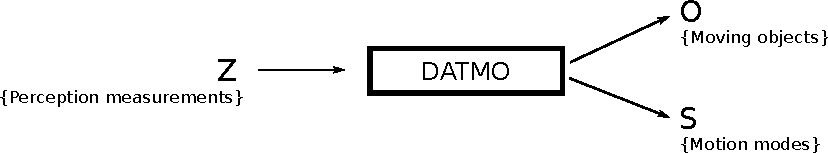
\includegraphics[scale=1.0]{img/fig:datmo:process}
     \end{tabular}
   \caption{DATMO process (adapted from \cite{Wang04a})}
   \label{fig:datmo:process}
 \end{figure}

Wang \cite{Wang03onlinesimultaneous} defined the DATMO tasks as:

\begin{itemize}
\item Detect and initializa new objects;
\item Motion modeling;
\item Data association;
\item Merge coalescent objects;
\item Remove the objects that moved outside of the FoV of the sensor;
\end{itemize}

Researchers considered SLAM and DATMO as two independent and different problems that should be solved separately. \textit{Wang} was the first researcher to put in evidence the similarities between both problems and propose simultaneous processing of those tasks\cite{Wang03onlinesimultaneous}. The SLAM and DATMO mutual cooperation is depicted in the Figure~\ref{fig:datmoslam:loop}.

\begin{figure}[h]
   \centering
     \begin{tabular}{lr}
       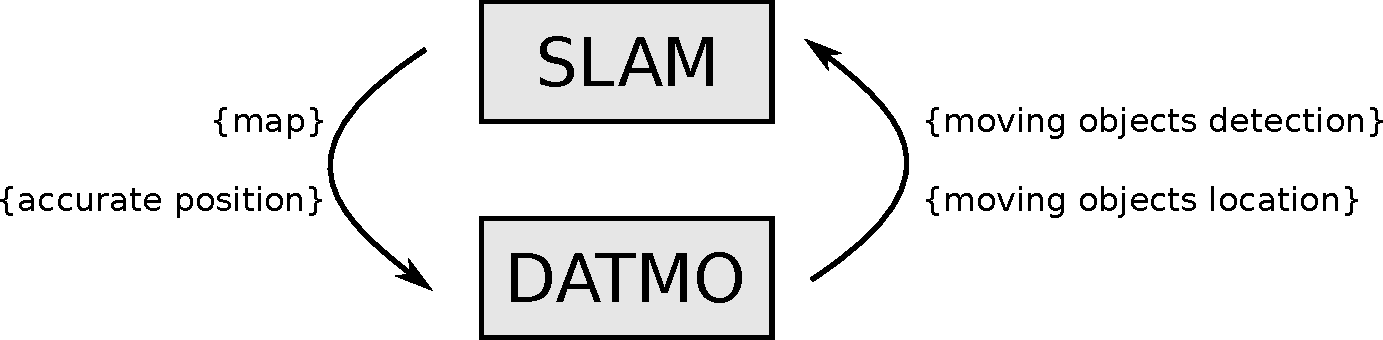
\includegraphics[scale=0.5]{img/fig:datmoslam:loop}
     \end{tabular}
   \caption{SLAM and DATMO: Mutual benefit (adapted from \cite{VU-2009-454238})}
   \label{fig:datmoslam:loop}
 \end{figure}

As result, the SLAMMOT term was coined and a derivation of the SLAM formula with DATMO was created to simplify the process of tracking. The experiments showed that solving simultaneously the SLAM with DATMO increased the quality of the algorithm results comparing them with their results as individual processes \cite{Wang02simultaneouslocalization}. In the other hand, the process gets much more complex and computational expensive. In the figure \ref{fig:slammot} we can see the input-process-output schema for the SLAMMOT process.

\begin{figure}[h]
   \centering
     \begin{tabular}{lr}
       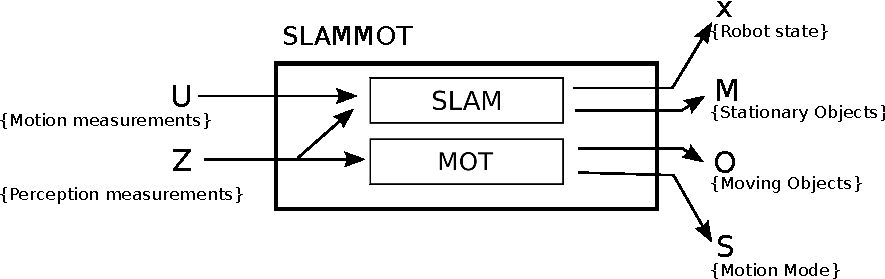
\includegraphics[scale=0.9]{img/fig:slammot}
     \end{tabular}
   \caption{SLAMMOT composition (adapted from \cite{Wang04a})}
   \label{fig:slammot}
 \end{figure}

Nowadays, the challenging in DATMO is to turn it into a reliable process in a highly dense and highly dynamic environments.

\section{Mutual cooperation: SLAM and DATMO}

\textbf{Scenario 1}: in a simpler scenario we can have a robot that moves in an environment, where all objects in its surroundings are static. The robot is the only element present in the environment that is moving.

In this case, the static environment is everything that the robot can perceive. So the robot should use these information to build a map of the navigable path (SLAM).

\textbf{Scenario 2}: suppose the robot is moving in an overly crowded environment, with different type of objects (cars, pedestrian, trucks, bicycle, motorbikes, etc.), static and moving objects are mixed. Which object to use as static objects (\textit{e.g.} to build the map) and which to use as dynamic (\textit{e.g.} to calculate the risk of collision)? 

In the \textbf{Scenario 2}, it is much more complicated to obtain any information from the environment.

This leads us to one conclusion: it is hard to do risk analysis when you do not know the objects of the scene. In addiction, it is intrinsically hard to find the motion model of a specific object in the scene(behavior analysis).

Thus, as a stepping stone we can perform the dynamic and static environment classification. This solves part of the problem, by classifying the environment in two categories. This will help to:

\begin{enumerate}
\item Build the map (which is not the our goal)
\item Perform DATMO
\item Perform risk assessment (Section~\ref{sec:riskassessment})
\end{enumerate}

The scene understanding usually implicates in distinguish different elements in the scene, objects or even types of objects. This distinction can be done by using the objects' features(\textit{e.g.} color, shape, etc.), path perceived or even its behavior (motion pattern behavior). 

\section{Problem addressed}

In this chapter we have seen the concepts required to understand the applicability of the problem addressed in this document. We introduced the most common approaches and terminologies adopted in the robotics field. 

In this document we will detail our approach to perform a fast and high level classification. Classifying dynamic parts in an image by using the minimum amount of video frames. The details of our methods will be explained in next sections.

%multimodels, importance sampling, prior map knowledge

%=====================
	
\chapter{State of the art}
	
There have been several proposals for classification methods, all on behalf of scene understading. Due to the variety of sensors and problem to takle, the techniques varies. The techniques are adapted accordingly.

The work over this theme copes with classification by establishing some ground-rules, the constraints in which the method relies on to work.

\section{Grouping issues in robotics}

One important step in the scene understanding is the environment map building and locate the ego-robot inside this map. This problem is known as SLAM \cite{Leonard2002Mobile}, which stands for Simultaneous Localization and  Mapping.

SLAM is composed of several steps to reach its goal: landmark extraction, data association, state estimation, etc. Each of them can be solved using different techniques.

SLAM tackles one specific scenario. SLAM assumes static environment constraint, in another words, any moving object in the same environment as the robot will interfere in the mapping process. For this reason, there is another process called DATMO to deal with the dynamism of the environment.

DATMO stands for Detection and Tracking of Moving Objects. When dealing with mobile robots in a dynamic environment we apply the DATMO process to obtain the moving objects from the environment.

\section{Solutions for segmentation}

\subsection{Stereo-visio camera}

In the Henning Lategahn and Bernd Kitt work \cite{DBLP:conf/ivs/LategahnGHKE11}, they proposed a classification method using stereo vision. Their work was evaluated theoretically by simulation and pratically by running the method in real footage from a moving vehicle.

One of the test cases had shown the capability of classification between the static and dynamic environment. In some situations the observation time had to be longer in order to perform correctly the classification. One of the reasons for that is the Sequential Probability Ratio Test (SPRT) performed in the samples.

Although the goal is the same in their and our work - classification - our method uses only LIDAR and IMU information to perform such classification.

\subsection{Single mono-vision camera}

In the work developed by Migliore et al. \cite{Migliore_2009_ICRA} is a MONOSLAM.. 

\subsection{LIDAR aproaches}

In the work \cite{4650636}, they use the Iterative Closest Point (ICP) \cite{10.1109/34.121791} to establish the displacement of the objects. 

This is difference in our method, first of all, we do not cluster to establish the boundaries of an object, this is not concerned by our application. For this reason we use grid based representation without clustering the objects, this was chosen due to it is parallelization and consequently it is speed.

We replaced the ICP algorithm by IMU measurements. The IMU measurements provide a approximate displacement of the vehicle, and based on that information we can calculate the displacement of the static objects in the scene.  


%=====================

\chapter{Motion Detection}
	%not in details put in introduction

\section{Introduction}

The main goal of this research is to distinguish all dynamic objects present in the scene. The scene is observed from a camera installed in a vehicle, so called testbed.

This setup brings one big issue: non-static sensor. Thus, \textit{apriori} all the objects are moving from the sensors perspective, even the static objects, due to the motion performed by the vehicle.

The distinction between static and dynamic are considering the subjects in a global reference frame, so the goal is to be able to classify the dynamic parts in the scene using the world as reference frame. By finding the dynamic parts $O_{dynamic}$ we can perfectly obtain the static $O_{static}$ ones as well, by subtracting the dynamic one from the scene $S$.

\begin{equation}
S=O_{static}+O_{dynamic}
\end{equation}

\section{Demonstrator configuration} %configuration of the lasers, diagram
\label{sec:demonstrator}

\subsection{LIDAR laser scanners}

Our testbed is a Toyota Lexus car equipped with two LIDAR lasers scanner (Check Section~\ref{sec:testbed} for the specification) installed in the frontal bumper (Figure~\ref{fig:demonstrator:birdeye}).

\begin{figure}[h]
   \centering
     \begin{tabular}{lr}
       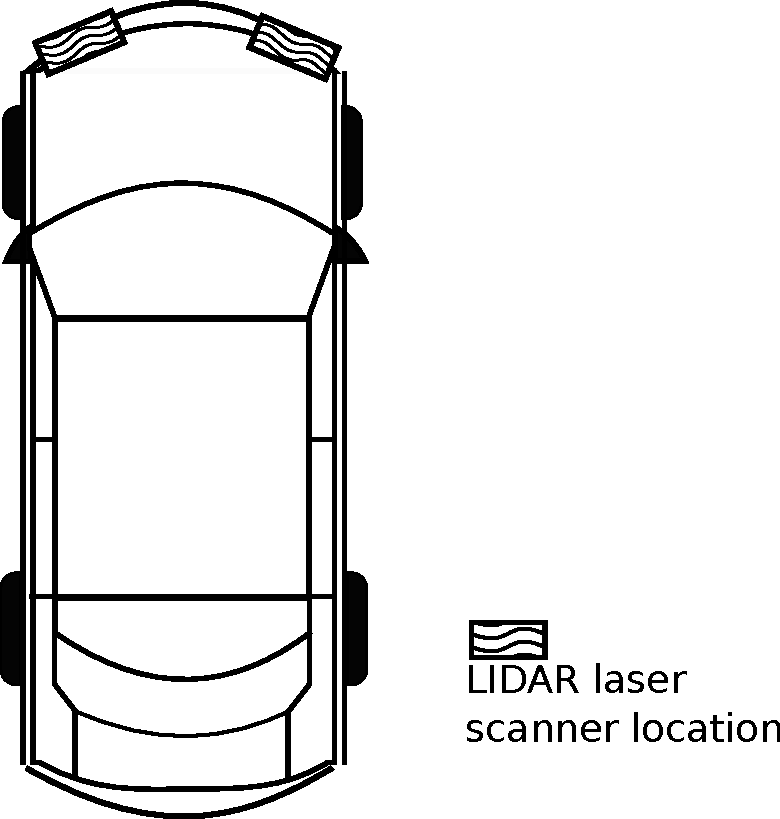
\includegraphics[scale=0.3]{img/fig:demonstrator:birdeye}
     \end{tabular}
   \caption{Bird-eye view: LIDAR laser scanners location}
   \label{fig:demonstrator:birdeye}
\end{figure}

Each LIDAR is capable of scanning in four layers, their relationship is shown  in the Figure~\ref{fig:demonstrator:lateral}, and every layers have its horizontal Field of View (FoV), one example is given for the layer 1 in the Figure~\ref{fig:demonstrator:superior}.

With four layers in total, the layers are arranged as planes with different angles but one common vetex, anchored at center of the LIDAR. The road is considered as base for the angle formation, it is formed with an imaginary plane, parallel to the road surface, and the a plane formed by the layer. Those angles are depicted in the Figure~\ref{fig:demonstrator:lateral}.

\begin{figure}[h]
   \centering
     \begin{tabular}{lr}
       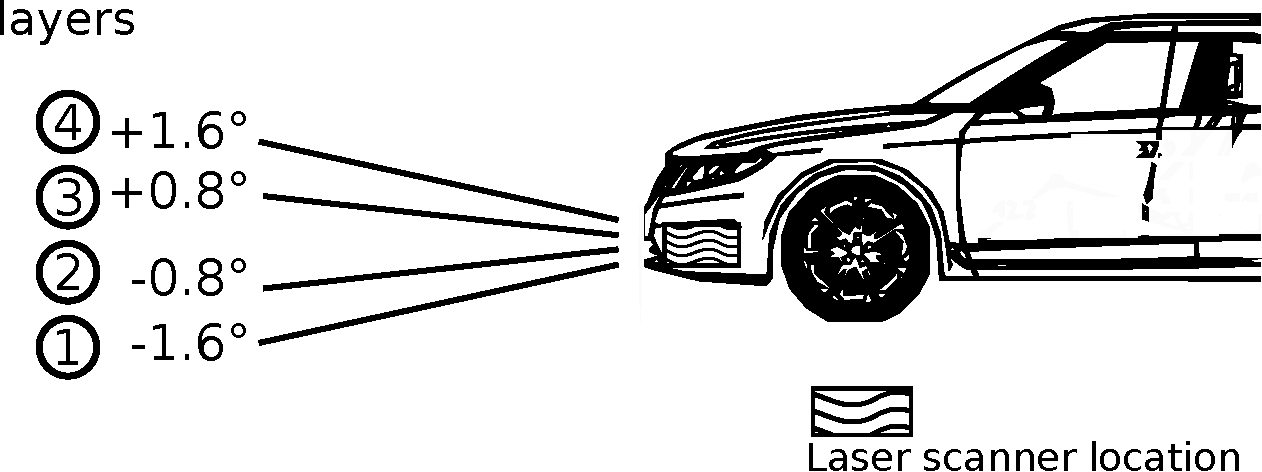
\includegraphics[scale=0.5]{img/fig:demonstrator:lateral}
     \end{tabular}
   \caption{Lateral view: Four layers of the left LIDAR laser scanner}
   \label{fig:demonstrator:lateral}
\end{figure}

A single layer sweeps the environment in a limited horizontal FoV, in the Table~\ref{tab:beam:interception} we can have the layers and their specific FoV. The LIDAR laser scanner, used in our tests, have the $0.5^{\circ}$ resolution. Meaning that every layer is capable of collecting samples at $0.5^{\circ}$ of angular distance in between. 

To calculate the number of beams available in a layer $\ell$ we apply the Equation~\ref{eq:totalbeams}, where the functions $min$ and $max$ are the minimum and maximum angles that can be reached by the layer $\ell$, and the function $resolution$ gives the resolution of the LIDAR laser scanner $\rho$, this is a specification provided by the manufacturer. 

Thus, we can calculate the number of beams in a layer based on its horizontal FoV and LIDAR resolution. Let's take as an example the first layer (layer 1) and calculate the number of beams available in this layer. 

The first layer (layer 1) has a horizontal FoV that varies from $+35^\circ$ to $-60^\circ$ (minimum and maximum FoV, respectively), the resolution of the LIDAR is $0.5^\circ$, according to the specification of the manufacturer. By applying those values in  the Equation~\ref{eq:totalbeams} we have as result $190$ beams available for the first layer.

\begin{equation}
\label{eq:totalbeams}
beams_{total}(\ell)=\frac{|max(\ell)-min(\ell)|}{resolution(\rho)}
\end{equation}

From every individual beam is possible to obtain the \textit{impact point}, meaning the distance between the LIDAR laser scanner and the first object to intercept the laser beam, limited to $200m$ maximum (More details about the specification in Section~\ref{sec:testbed}).

\begin{figure}[h]
   \centering
     \begin{tabular}{lr}
       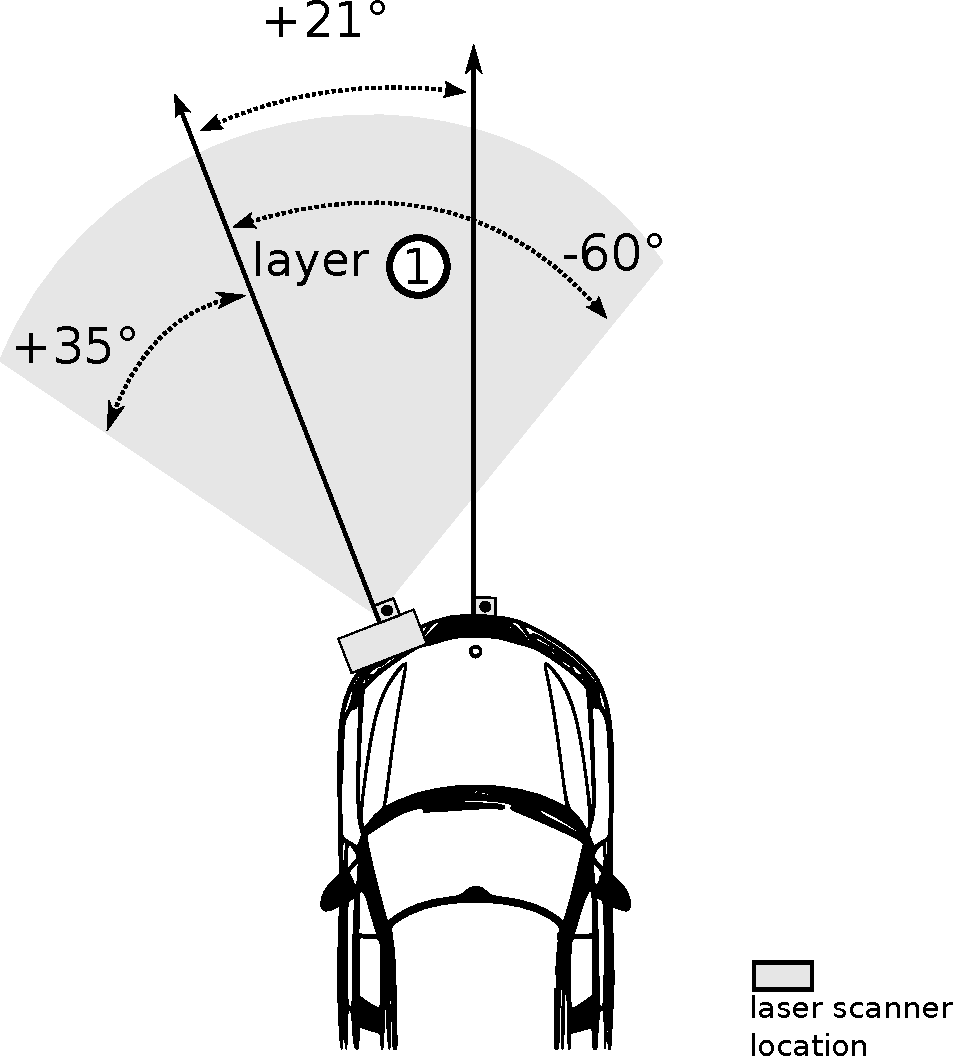
\includegraphics[scale=0.5]{img/fig:demonstrator:superior}
     \end{tabular}
   \caption{Bird-eye view: Left LIDAR laser scanner FoV, for the first layer}
   \label{fig:demonstrator:superior}
\end{figure}


\begin{table}
	\begin{center}
	    \begin{tabular}{ | c | c | c | c | c |}
		    \hline
		    Layer & $+50^\circ$ to $+35^\circ$ & $+35^\circ$ to $-50^\circ$ & $-50^\circ$ to $-60^\circ$ \\ \hline
		    4 & + & + &    \\ \hline
		    3 & + & + &    \\ \hline
		    2 &  & + & + \\ \hline
		    1 &  & + & + \\ \hline
		    $\cap$ &  & + &   \\ \hline
	    \end{tabular}
	\end{center}
    \caption{Layers and the horizontal distribution of the beams}
\label{tab:beam:interception}
\end{table}

The multiple sensor usage in the demonstrator car makes of it a complex system, due to the number of data gathered, overlapped information and possible conflicted data (Figure~\ref{fig:demonstrator:superior:overlap}). Thus, all sensor information must be carried in a consistent manner and this is accomplished by fusing the sensor information, more details about how this is done in the Section~\ref{sec:sensor:fusion}.

\begin{figure}[h]
   \centering
     \begin{tabular}{lr}
       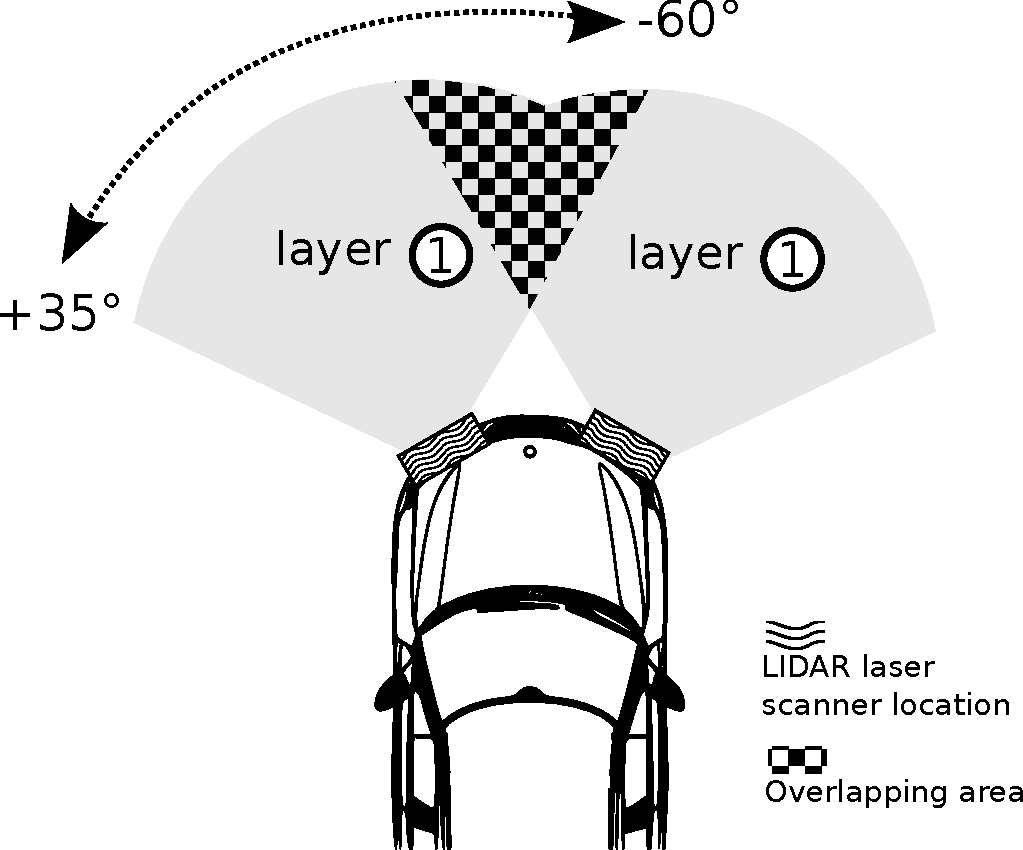
\includegraphics[scale=0.5]{img/fig:demonstrator:superior:overlap}
     \end{tabular}
   \caption{Bird-eye view: LIDAR overlapping area}
   \label{fig:demonstrator:superior:overlap}
\end{figure}

In the Figure~\ref{fig:demonstrator:superior:overlap} we depict the overlapping area when we consider the two LIDARs installed in our testbed.

\subsection{MTi-G XSens}

As we are about to see in the next Sections, the algorithm developed in this document uses two main data as input: the LIDAR data (explained previously) and MTi-G sensor data.

\begin{figure}[H]
   \centering
     \begin{tabular}{lr}
       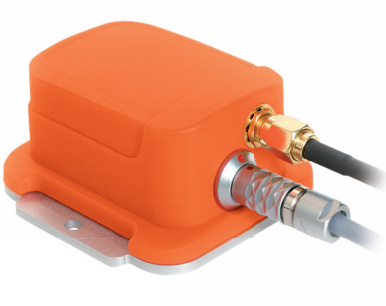
\includegraphics[scale=0.3]{img/mti-g}
     \end{tabular}
   \caption{MTi-G unit}
   \label{fig:xsens:mtig}
 \end{figure}

MTi-G unit (Figure~\ref{fig:xsens:mtig}) is a combination of Inertial Measurement Unit (IMU), GPS and barometer. The concept of MTi-G unit is not just gathering a set of sensors, it is about using information among them so that each individual sensor information can get benefits from the other ones and provide more precise information.

One example good example is that the GPS can use the other sensor to estimate the position, this is useful in case of a short-period communication outages, giving the global position estimation even without GPS signal. 

From this sensor unit our algorithm utilizes the vertical $v_y$ velocity, horizontal $v_x$ velocity and the $Yaw$ angle of the car. The $Yaw$ is the angle of the car with respect to some fix point in earth (\textit{e.g.} north oriented). The fix point is irrelevant, since we are concerned about the angle variation and not the exactly angles theirselves, as we are going to see in the Section~\ref{ch03:motiondetection}.

\section{Sensor pre-processing} %fusion module
\label{sec:sensor:fusion}

% in the last subsection, output form (occupancy grid), digrams; explains that this is our input

\subsection{Purpose}

The demonstrator car is composed with two LIDAR laser scanner sensors, as we saw in the Section~\ref{sec:sensor:fusion}. Each of the LIDAR laser scanner is composed of few layers and each layer contains several beams. Those beams are spread in a given horizontal FoV. The horizontal FoV is layer dependent, varying according to the layer.

In the Figure~\ref{fig:motion:framework}, we have represented the general framework modules for detecting the moving parts, our algorithm core is contained in the motion detection module, which will be explored later. We are making usage of two LIDARs, they provide several information from different specifications (different ranges and FoV), thus we use a fusion module which is responsible for gathering the information provided by all of the LIDAR in a consistent manner.

\begin{figure}[h]
   \centering
     \begin{tabular}{lr}
       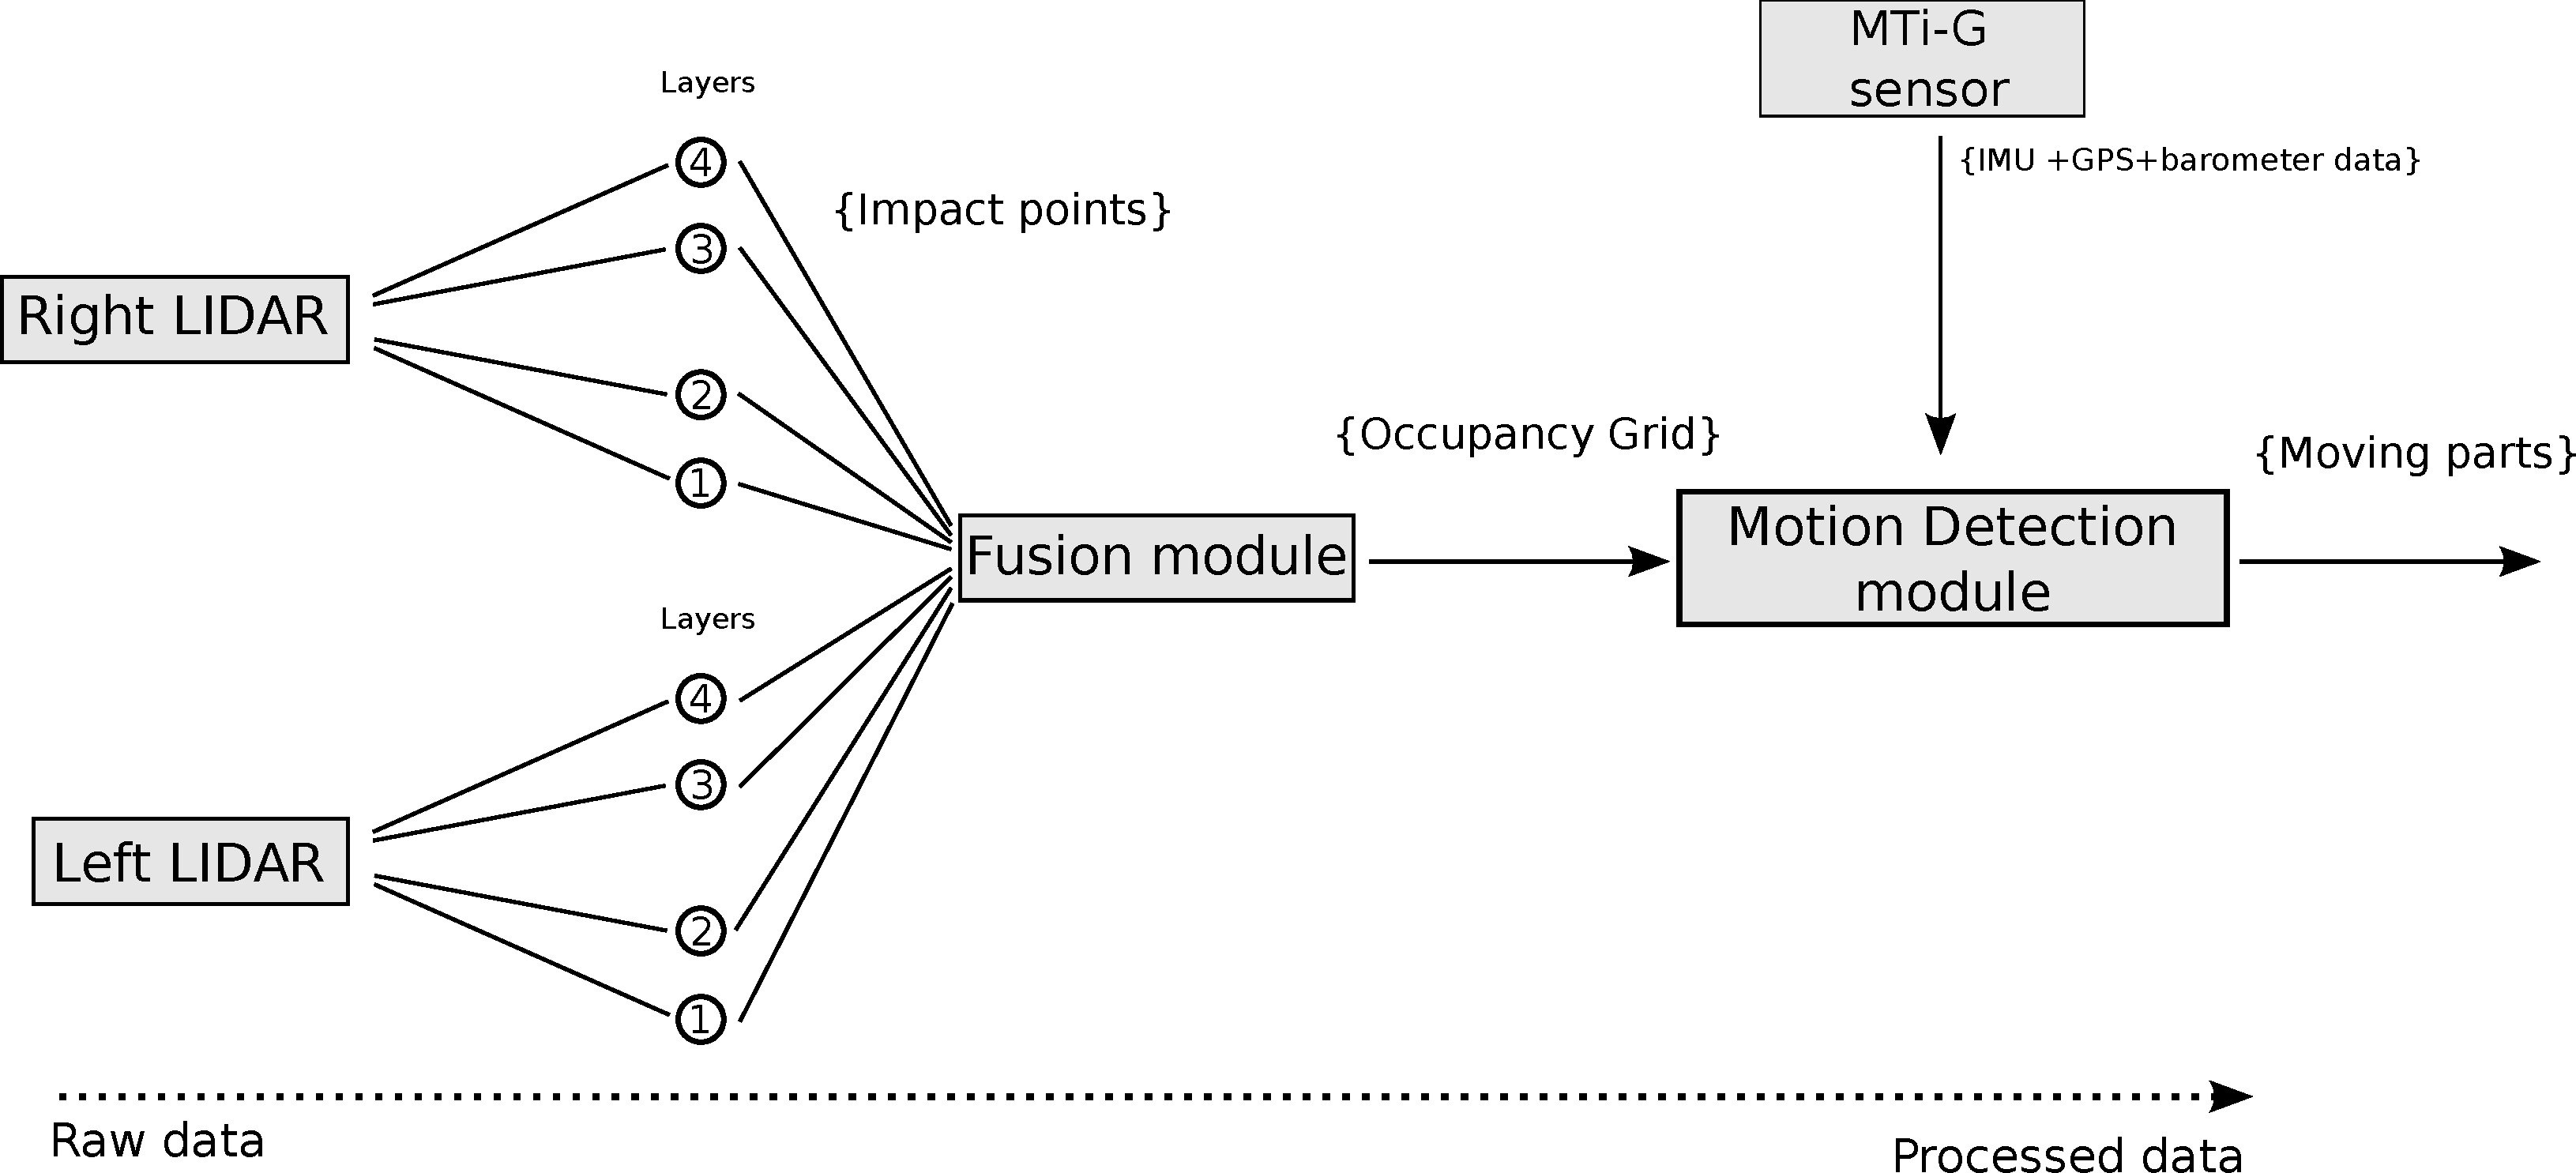
\includegraphics[scale=0.30]{img/fig:motion:framework}
     \end{tabular}
   \caption{General framework for detection of moving parts}
   \label{fig:motion:framework}
\end{figure}

This data must be gathered together, but how give a unique representation for all information provided by the sensors in one single visualization? Recall that there are overlapping scanner reading, which means that there may exist conflicting readings due to the sensor failure, or a bad environment condition.

Solving that issue implies in data fusion. \textit{Linear Opinion Pools} was used successfully by an INRIA team member to make data fusion, detailed information about this technique is explained in the document \cite{ADARVE-2012-671211}. The output of such fusing technique is an Occupancy Grid, which is used by our algorithm.

\subsection{LIDARs layers fusion}

\subsubsection{Sensor fusion from the multiple lidar layers}
Each of the  two LIDAR sensors installed on the vehicle provides us 4 layers of impact points. Each layer is used to compute an occupancy grid using the classical approach described in \cite{Thrun05}. In order to retrieve a single grid for representation of the environment, the data from all these layers are merged using the approach described in \cite{ADARVE-2012-671211}. This approach fuses the sensory information by using Linear Opinion Pools \cite{DeGroot1974}. It has the advantage of reducing the errors generated by conflicting information from the multiple layers.

The principle is to generate a posterior distribution over the occupancy of a cell $C$ of the grid given the opinion of $m$ sensors $\left\{ Y_1 \dots Y_m \right\}$.
Each sensor gives two quantities: its estimation for the occupancy of the cell $P(C | Y_i)$ and the confidence weight $w_i(C)$.
The idea is to shut-down those sensors that do not give relevant information to the process by assigning a low weight to them. The fusion of all sensory information will be as follows:

\begin{equation}
\label{linealOpinionPoolEQ}
  P(C | Y_1 \dots Y_m) = \alpha \sum \limits^m_{i=1} w_i(C) P(C | Y_i)
\end{equation}
Where $\alpha = \left[ \sum \limits^m_{i=1} w_i(C) \right]^{-1}$ is a normalization factor for the weights.  Equation \eqref{linealOpinionPoolEQ} is used to generate
2D-occupancy grids. For each sensor $Y_i$ we must define $P(C | Y_i)$, the probability of a cell being occupied given the sensor information. Complete derivations for these quantities are provided in \cite{ADARVE-2012-671211}. The output of this fusion module is an occupancy grid. %write about occupancy grid

Note that we assume independence among cells. This assumption is very strong, although it is necessary so the computation of the Equation~\eqref{linealOpinionPoolEQ} be efficient, by computing each cell value in parallel. %add section about performance

\subsubsection{Justifying the performance}

The independence among the cells is the main responsible for the high level of parallelism in the algorithm, the high level of parallelism and the performance can be assured by \textit{Amidahls law}.

\textit{Amidahls law} is a diminishing return law. It states that the gaining in performance (speedup) is not necessarily in the same magnitude as the number of new workers added for the execution of the algorithm\cite{Amdahl:1967:VSP:1465482.1465560}. This is pretty much saying that one adult female can have one children in 9 months but two adult female cannot have one children in 4.5 months, it always depends if the task can be really accomplished in parallel, of course this is an simplistic view, but gives you an idea.

In the Equation~\ref{eq:amidahls}, Amidahls describes the time to execute an algorithm in parallel ($T_p$). Its execution time depends on the time required by sequential part of the algorithm ($T_{seq}$, part which can not be parallel) along with the time for part of the algorithm that can be parallel($T_{par}$) divided by the number of workers ($p$, \textit{e.g.} number of cores in a multi-core processor).

\begin{equation}
\label{eq:amidahls}
T_p=T_{seq}+{T_{par} \over p}
\end{equation}

As in our case the cells are completely independent, the gaining in parallelization is maximum since the term $T_{seq}$ is zero (the sequential code is inexistent), and the processing time is divided among the workers.

\section{The algorithm}
%motion detection

\subsection{Principle} 

\textit{Frame} is a snapshot of the current environment representation, it is used as one of the inputs for the algorithm developed in this work.

But before jump on explanations on how the frames are going to be used, we need to describe how those frames are obtained and how do they mimic the environment.

In the Section~\ref{sec:demonstrator}, we saw that our testbed is composed by two scanners, each of them containing several layers. Every layer has a certain number of beams, which are distributed in the horizontal FoV within a regular angle interval. 

So, before having a frame that can be used by our algorithm, it is required to perform the fusion of the layers from the LIDAR, which is done by the \textbf{fusion module}. 

The details about the techniques adopted and the data processing were explained in the Section~\ref{sec:sensor:fusion}. From here on, we are going to proceed with explanation of our methods, which is identified as \textbf{motion detection module}. This module is located at the end of the processing chain, as exhibit in the Figure~\ref{fig:motion:framework}. 

\begin{figure}[h]
   \centering
     \begin{tabular}{lr}
       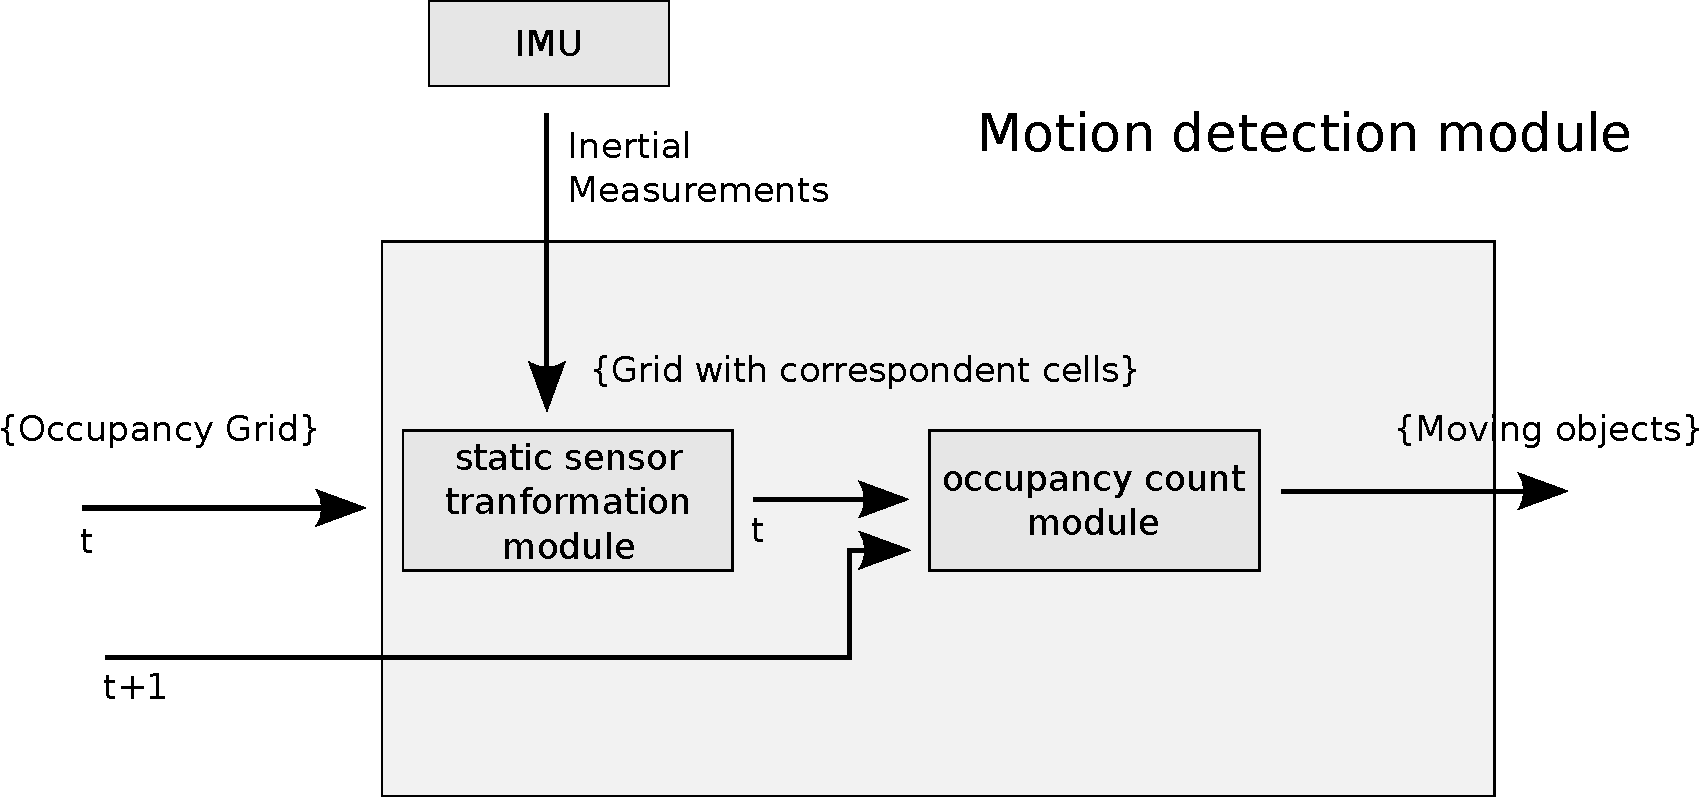
\includegraphics[scale=0.50]{img/fig:motion:framework:motionmodule}
     \end{tabular}
   \caption{Motion detection module anatomy}
   \label{fig:motion:framework:motionmodule}
\end{figure}

%%%%%%%%%%%%%%%%%%%%%%%%%%%%

\subsection{Non-static sensor issue}

The LIDAR is installed on a vehicle, the goal is to acquire measures while vehicle is moving. So it captures the surrounding and the data is processed by the \textbf{fusion module} resulting in Occupancy Grid $OG_t$. This process is repeated for each frame obtained. This is required to transform the data into the proper input for \textbf{motion detection module}.

The position of the LIDAR gives us the fully dynamic scenario impression. Meaning that, by the LIDAR sensor perspective the entire scenario is moving and all subjects are changing their position, except for those who are following the same trajectory as the vehicle and at the same speed. 

The LIDAR can read informations from the environment with $25fps$. Although, we are able to achieve good qualitative results using a short amount of frames. 

Due to the good qualitative results obtained by using the two frames approach, we will demonstrate all formulas by considering such configuration - only two frames for the calculation. But we may reference other frames in exploratory examples.

% & 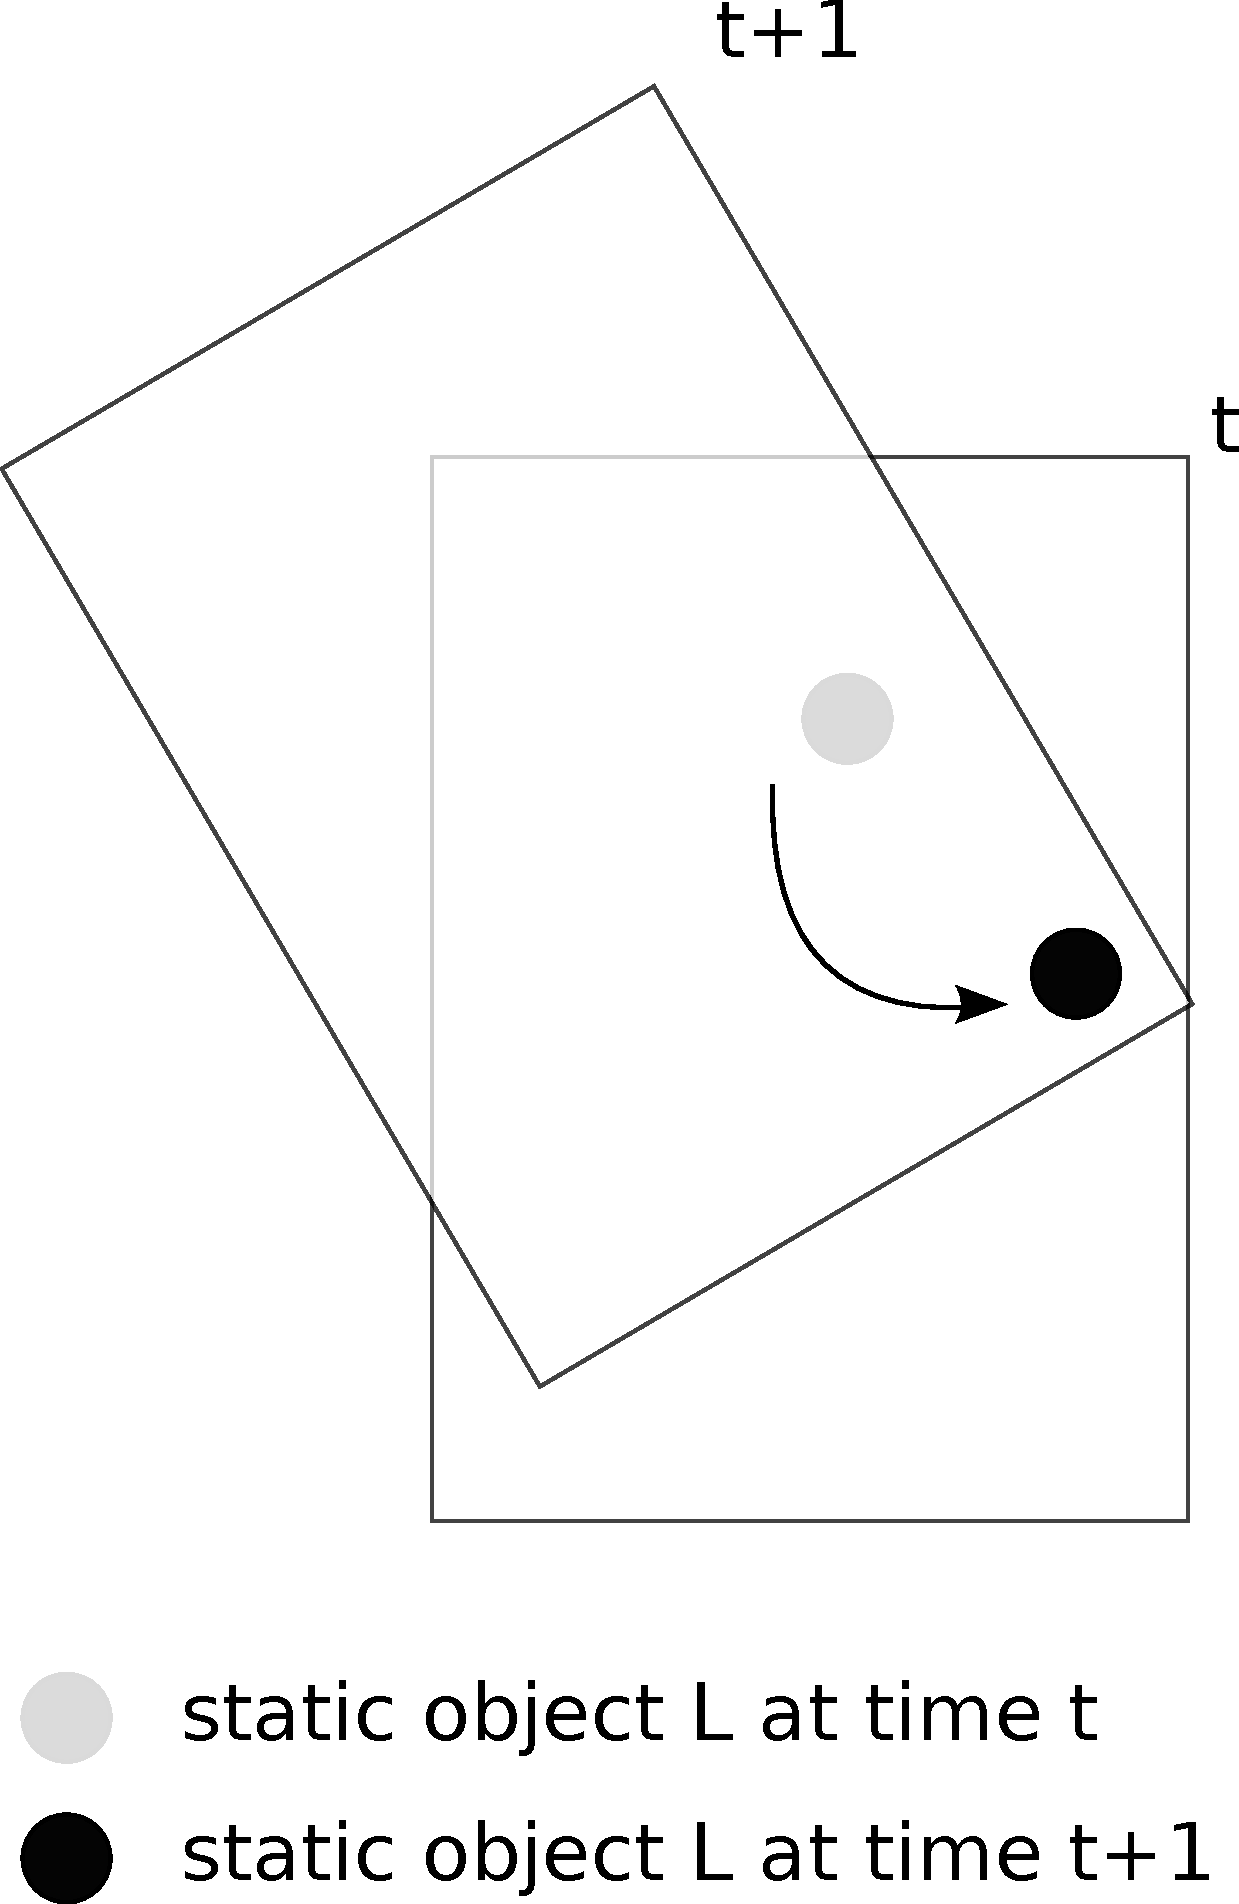
\includegraphics[width=0.3\columnwidth]{img/fig:motion:algorithm:nonstatic:02}

\begin{figure}[h]
   \centering
     \begin{tabular}{lr}
       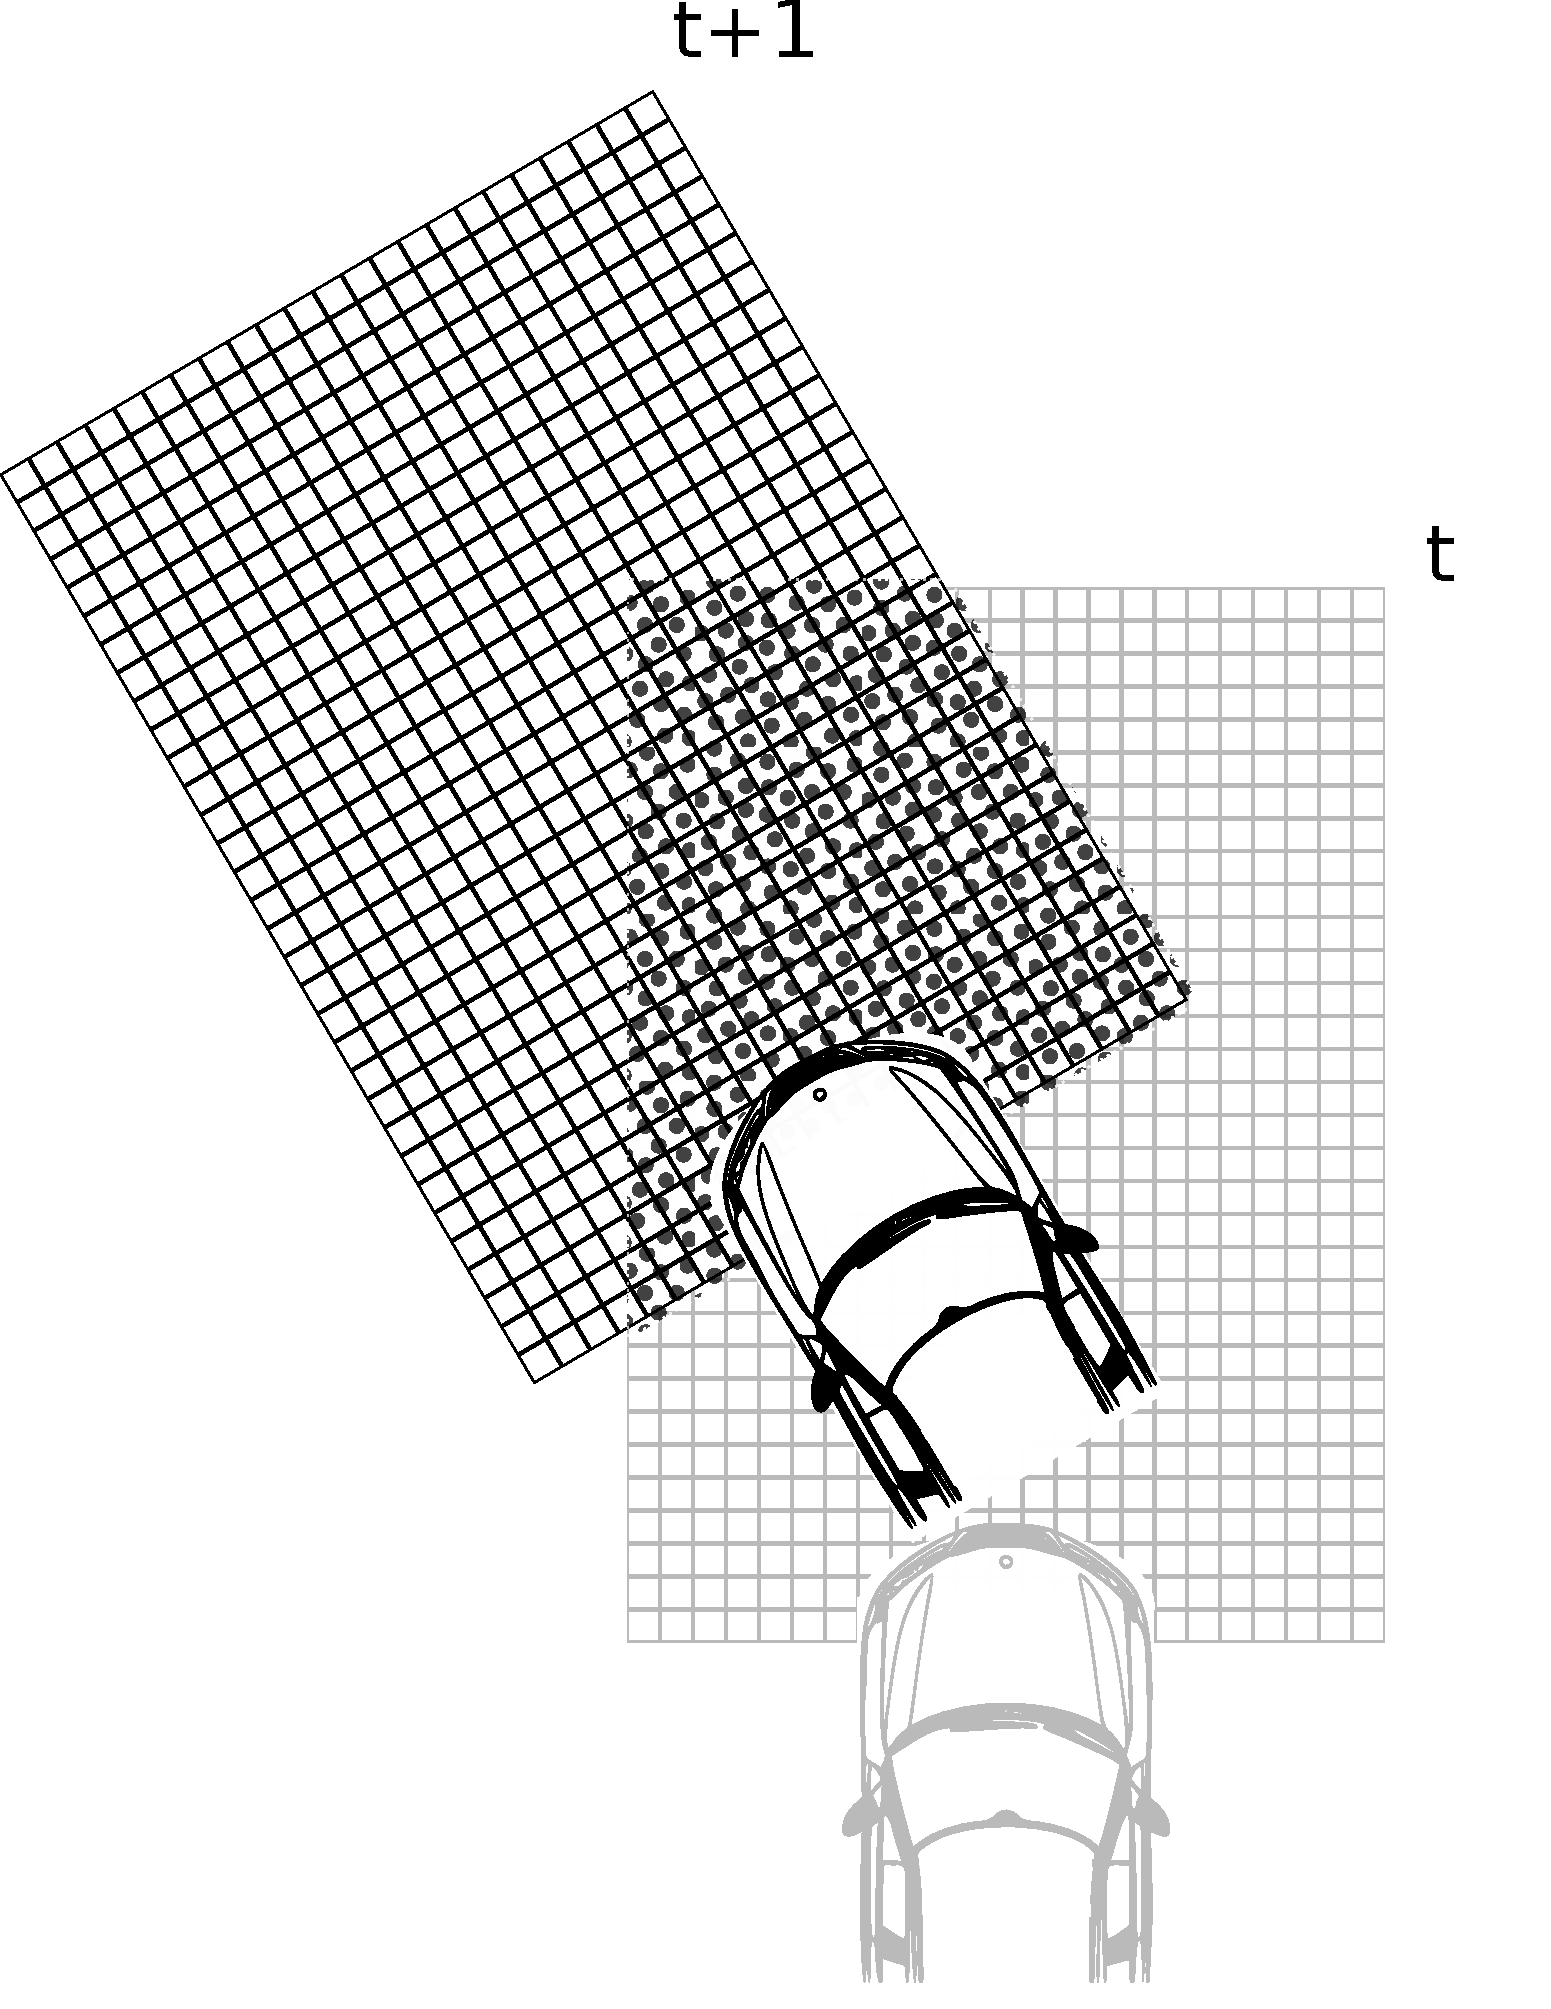
\includegraphics[width=0.35\columnwidth]{img/fig:motion:algorithm:nonstatic:01}
     \end{tabular}
   \caption{frames $f_t$ and $f_{t+1}$ with the intersection area}
   \label{fig:motion:algorithm:nonstatic:01}
 \end{figure}

The method developed in this document initially requires a static sensor, this constraint assumes that there is an exact correspondence between the cells among frames. Such constraint is not true in our application since the goal is to have it running in a moving vehicle, as an ADAS application. 

To better understand this issue take a look at the example: assume our vehicle is driving along a street and makes a left turn, we capture two frames, one while the car was driving straight $f_t$, and the second frame  after the car initiate the left turn $f_{t+1}$. We observe an a static object in the frame $f_t$ (\textit{e.g.} telephone pole in the sidewalk) that was located at $d_t$ meters from the car, and in the frame $f_{t+1}$ this very same object will be at $d_t-\Delta d(f_t,f_{t+1})$ and will be slightly moved to the right side (due to the left turn). The function $\Delta d$ returns the distance traveled by the car between the two frames. This behavior can be seen in the Figure~\ref{fig:motion:algorithm:nonstatic:01}, and as we can see, we can extract informations only from overlapping areas between two frames(Figure~\ref{fig:motion:algorithm:nonstatic:01} dotted area in the left image), but since this analysis is done in very small time variation, we have a great portion of overlapping area.

This problem is solved by introducing the Inertial Measurement Unit(IMU) data. The IMU provides information about the inertial behavior of the unit. Although not all information generated by the IMU are needed, the ones used are speed $s$, yaw angle, vertical $v_v$ and horizontal $v_h$ velocity. Those informations are used to apply the necessary transformation to the $f_t$ making its cells match the cells $f_{t+1}$. Thus finding the correspondence between cells of $f_t$ and $f_{t+1}$.

From the IMU information we calculate two parameters: angular velocity and the linear velocity. 

Angular velocity is obtained by finding the angle variation between the frames $f_t$ and $f_{t+1}$, according to the Equation~\ref{eq:angularvelocity}, $\Delta t$ represents the time variation between the frames.

\begin{equation}
\label{eq:angularvelocity}
\omega(f_t,f_{t+1}) = \frac{Yaw_{t+1}-Yaw_t}{\Delta t(f_t,f_{t+1})} 
\end{equation} 

The angular velocity is given in degrees, but the IMU gives us a quaternion for the angle of the vehicle. The quaternion is the most common way to represent angles in 3d world, due to the fast calculations and it solves the gym ball lock problem, which is common for euler angles. Converting the value from quaternion to Euler angles is straightforward by the Equation~\ref{eq:quaternion}.

\begin{equation}
\label{eq:quaternion}
Yaw=atan2(2(q_0 q_3+q_1 q_2),1-2(q_2^2+q_3^2))
\end{equation}

The angular velocity $\omega(f_t,f_{t+1})$ is used to adjust the angle of $f_t$, put this value aside, before apply this transformation to the frame $f_t$ we have to calculate the displacement of the grid.

At this point, we have the information about the proper angle for the frame $f_t$, the next step is to calculate the displacement of the frame. The displacement is calculated based on the actual velocity of the vehicle at the time $t$. 

The IMU keeps the velocity in two components, the horizontal $v_h$ and vertical $v_v$ velocities, and to obtain the actual velocity, we can apply the Equation~\ref{eq:velocity}, which extracts the velocity based on the two components.

\begin{equation}
\label{eq:velocity}
v_t=\sqrt{v_h^2+h_v^2}
\end{equation}

\subsection{Motion detection}
\label{ch03:motiondetection}

In this section we going to detail the technique that we developed to find moving parts of the environment. 

The input to this motion detection module consists of an occupancy grid and the vehicles velocities. The occupancy grid is generated by the fusion module described in previous section and that fuses data from eight layers of two laser scanners installed on the demonstrator vehicle. The vehicles velocities are provided by the MTi-G sensor unit.

Let us represent this occupancy grid at time $t$ as  $OG_t$. The value of each cell of this grid is between 0 and 1 i.e. $0 \leq OG_t[i] \leq 1$ (where $0 \leq i<N$ with $N$ being the total cells of this occupancy grid) which represents internal belief of the ego vehicle about the occupancy state of each cell where 0 means empty and 1 means occupied.

%explain XSens MTI-G in the beginning LIDAR, SENSOR MTI

The output of the \textit{XSens MTI-G} sensor, at time instant $t$,
consists of (along with other information) two components of velocity $v_t=(v_x, v_y)$ and values of
quaternion components for orientation $Q_t=(q_0, q_1, q_2, q_3)$. From those information we calculate the
translational and rotational velocities are represented by the tuple $u_t=(\nu_t, \omega_t)$, the velocity is calculated according to the Equation~\ref{eq:ch03:velocities}.

\begin{equation}
\label{eq:ch03:velocities}
\nu_t = \sqrt{v_x^2+v_y^2}
\end{equation}

To calculate rotational velocity of the vehicle we calculate yaw angle of the vehicle from the quaternion
as demonstrated in the Equation~\ref{eq:quaternion:yaw}, the $Yaw$ will be given in radians.

\begin{equation}
Yaw = atan2(2(q_0 q_3+q_1 q_2),1-2(q_2^2+q_3^2))
\label{eq:quaternion:yaw}
\end{equation}

And if $\Delta t$ is the time difference between two data frames at time $t$ and $t-1$ then rotational speed $\omega$
at time $t$ is equal to the yaw rate given as:
\begin{equation}
\omega_t = \frac{Yaw_t-Yaw_{t-1}}{\Delta t}
\end{equation}

At each time instant $t$ these $OG_t$ and $u_t$ are input to the algorithm that consists of 
following steps.

\paragraph{Free and occupied counters arrays} for each new input occupancy grid $OG_t$ we 
create two parallel counter arrays, having the same size ($N$ cells) as $OG_t$. The first called $FreeCount_t$ and the other called $OccupiedCount_t$ to keep the count of the number of times that a cell has been observed free and number of times it has been observed occupied, respectively. These arrays are initialized from $OG_t$ as follows ( $\forall i$  . $0 \leq i<N$ ):

\begin{equation}
OccupiedCount_t[i] =  \begin{cases} 1, & \mbox{ if $OG_t[i] > 0.5$} \\
                       0, & \mbox{otherwise} \end{cases}
\end{equation}
and
\begin{equation}
FreeCount_t[i] = \begin{cases} 1, & \mbox{ if $OG_t[i] < 0.5$} \\
                       0, & \mbox{otherwise} \end{cases}
\end{equation}

\paragraph{Counts update from previous step} Suppose $FreeCount_{t-1}$ and  $OccupiedCount_{t-1}$ are the
updated counter arrays at time $t-1$ and we want to update new counters $FreeCount_t$ and $OccupiedCount_t$
from these old counts. Since vehicle has undergone a position change determined by $u_t=(\nu_t, \omega_t)$
so there is no direct correspondence between cells of two occupancy grids $OG_t$ and $OG_{t-1}$ and we
must find transformations that map a cell in  $OG_{t-1}$ to a cell in $OG_{t}$ using $u_t$. This situation is
shown in Figure \ref{fig:gridmove}, $OG_{t-1}$ has origin at $O_{t-1}$ and $OG_t$ has origin at $O_t$. To find this transformation suppose $O_{t-1}=(x_{t-1}, y_{t-1}, \theta_{t-1}) = (0,0,0)$ is the pose (position and orientation) of the occupancy grid at time instant $t-1$ (i.e in $OG_{t-1}$) and we want to find $O_t=(x_t, y_t, \theta_t)$, the pose of $OG_t$ with respect to $OG_{t-1}$ after it has undergone a motion of $u_t$. By taking $O_{t-1}=(0,0,0)$ in each iteration of the algorithm.

We highlight the fact that we solve localization only for two consecutives frames and do not care about the global localization. 

Now if $\Delta t$ is the time difference between the instants $t$ and $t-1$ then using circular motion model the pose $O_t$ is given as:

\begin{equation}
\left[\begin{array}{c}x_t \\ y_t\\ \theta_t \end{array} \right] = 
\left[\begin{array}{c} {\nu_t \over \omega_t} \sin(\omega_t \Delta t) \\ {\nu_t \over \omega_t} - {\nu_t \over \omega_t} \cos(\omega_t \Delta t) \\ \omega_t \Delta t \end{array}\right]
\end{equation}

\begin{figure}[h]
\begin{center}
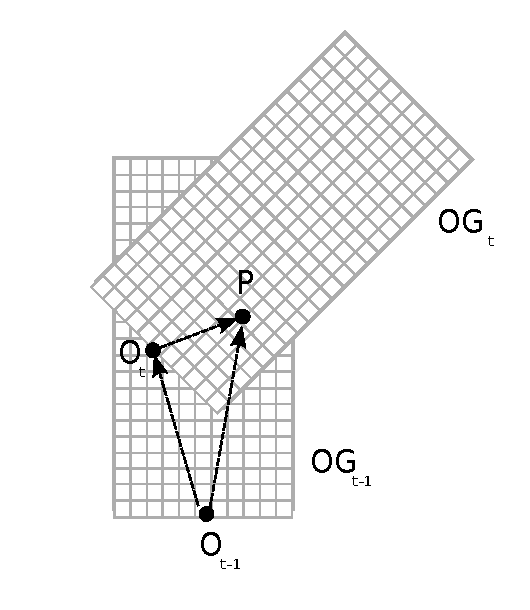
\includegraphics[scale=0.8]{img/fig:translation}
\caption{Position of the grid at instants $t-1$ and $t$. Vehicle undergoes a motion of $u_t=(\nu_t, \omega_t)$ to move from $O_{t-1}$ to $O_t$. We need to find the position of point $P$ of grid $OG_{t-1}$ in grid $OG_t$.}
\label{fig:gridmove}
\end{center}
\end{figure}

An important thing is to notice that we are concerned with the localization of two consecutive frames only
and need not solve the complete SLAM problem, making the technique very fast. Moreover, empirical observation suggests that the odometry error between two consective frames is less than 10 cm whereas the cell size assigned is $20cm \; x \; 20cm$ enabling us to assume that cell mapping (explained next) from grid at $t-1$ to grid at $t$ is exact.

Mapping a cell of the grid $OG_{t-1}$ to $OG_t$ consist in bring $OG_{t-1}$ up to speed based in the MTi-G sensor unit information. Suppose point $P$ (shown in Figure \ref{fig:gridmove}) is the center of a cell in grid $OG_{t-1}$ and we want to find its corresponding cell in grid $OG_t$. We define following two pose manipulation operations. if $P_{ij}=[x_{ij}, y_{ij}, \theta_{ij}]^T$ is the pose of origin $j$ w.r.t origin $i$ and $P_{jk}=[x_{jk}, y_{jk}, \theta_{jk}]^T$ is the pose of origin $k$ w.r.t $j$ then the pose of $k$ w.r.t $i$ denoted as $P_{ik}=[x_{ik}, y_{ik}, \theta_{ik}]^T$ is given as:

\begin{equation}
P_{ik} \equiv \oplus (P_{ij}, P_{jk}) = \left[ \begin{array}{c}
x_{jk}\cos(\theta_{ij})-y_{jk}\sin(\theta_{ij})+x_{ij} \\
x_{jk}\sin(\theta_{ij})+y_{jk}\cos(\theta_{ij})+y_{ij} \\
\theta_{ij}+\theta_{jk} \end{array} \right] 
\end{equation}

For the pose $P_{ij}$ the reverse pose relationship $P_{ji}=[x_{ji}, y_{ji}, \theta_{ji}]^T$ (pose of $i$ w.r.t $j$) is defined as:

\begin{equation}
P_{ji} \equiv \ominus (P_{ij}) = \left[ \begin{array}{c}
-x_{ij}\cos(\theta_{ij})-y_{ij}\sin(\theta_{ij}) \\
x_{ij}\sin(\theta_{ij})-y_{ij}\cos(\theta_{ij}) \\
-\theta_{ij} \end{array} \right] 
\end{equation}

Since the pose of $O_t$ w.r.t $O_{t-1}$ is $P_{O_{t-1}O_t}=[x_t,y_t,\theta_t]^T$ and point $P$ has pose $P_{O_{t-1}P}=[x,y,0]^T$ w.r.t $O_{t-1}$. The pose of this point $P$ w.r.t $O_t$ is calculated as:

\begin{equation}
P_{O_tP} = \oplus (P_{O_tO_{t-1}}, P_{O_{t-1}P})
\end{equation}

or

\begin{equation}
P_{O_tP} = \oplus (\ominus(P_{O_{t-1}O_t}), P_{O_{t-1}P})
\end{equation}

First two components of $P_{O_tP}$ give $x$ and $y$ position of the point $P$ w.r.t origin $O_t$. From these $x$ and $y$ values we can easily calculate the index of the cell where point $P$ lies in grid $OG_t$. In the Equation~\ref{eq:grid:cell:calculation} we calculate the row and column of the cell in which $P$ lies, where $cell_{size}$ is $0.2m$ and $gridWidth$ is $20m$ .

\begin{equation}
cell(column,row)=\left\{\frac{1}{cell_{size}}(x+\frac{gridWidth}{2}),\frac{y}{cell_{size}} \right\}
\label{eq:grid:cell:calculation}
\end{equation}


%\begin{equation}
%cell_{column}=(x+gridWidth/2)/cellSize
%\end{equation}

%\begin{equation}
%cell_{row}=y/cellSize
%\end{equation}

These transformations will map a cell having index $i$ in $OG_{t-1}$ to a cell having index $j$ in grid $OG_t$. If this cell $j$ is visible in $OG_t$ i.e $0 \leq j<N$ then we can update new count values for this cell as follows:

\begin{equation}
FreeCount_t[j] = FreeCount_t[j] + FreeCount_{t-1}[i]
\end{equation}

and

\begin{equation}
OccupiedCount_t[j] = OccupiedCount_t[j] + OccupiedCount_{t-1}[i]
\end{equation}

We repeat this process for all cells of grid $OG_{t-1}$ to update counter values in grid $OG_{t}$.

\paragraph{Motion detection} After the counts arrays have been updated as explained above the motion grid can be calculated from the new data as follows:

\begin{equation}
MotionGrid_t[i] = \begin{cases} 1, & \mbox{$OG_t[i] > 0.5$ and} \\ & \mbox {$FreeCount_t[i]>2\;  x \; OccupiedCount_t[i]$} \\
                                0, & \mbox{otherwise}\end{cases}
\end{equation}
After this process, the $MotionGrid_t$ becomes a binary grid, where it has 1's assigned to the cells which belongs to moving parts, and 0's otherwise.

%%%%%%%%%%%%%%%%%%%%%%%%%%%%%%%%%%%%%%%%%%%%%%%%%%%%%%%%%%%%%%%%%%%%%%%%%%%%%%%%



%\subsection{Solution}


%\section{summary}

%summary

%=====================

\chapter{Implementation}
	\section{Experiment}

In the beginning of the experimentation phases, we modeled the algorithm to compute ahead of the time by using the bicycle model and extrapolating the pose by using the current vehicle measurements, like stearing angles. But this measurement had shown a lot of variation during a run, and the extrapolated model gets out to date very quickly.

From mechanical physics we obtain the angular velocity and from the vehicle \emph{CAN bus} we obtain the data time stamp, and along with it the time variation, $\Delta t$.

Using transformational matrices we bring the car perspective \cite{iyengar1991autonomous} and the prediction to the same frame of reference.

\section{Evaluation}

%target: dynamic and static separation, reduce the number of frames required, no classification, no association; no tracking, no 

\subsection{Testbed}

\subsubsection*{Hardware}

For testing purposes, we have a Lexus LS600h equipped with a stereo vision (TYZX camera) positioned in the superior part of the windshield.

The vehicle has two IBEO Lux Lidar in the front side of the car, one in each corner of the bumper.

As IMU, the car is equipped with a Xsens IMU and a GPS for global positioning.

\begin{figure}[h]
   \centering
     \begin{tabular}{lr}
     \multicolumn{2}{c}{ 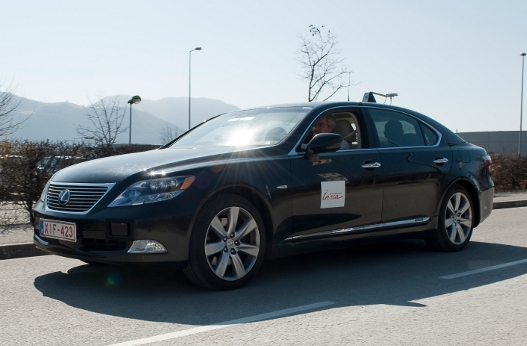
\includegraphics[width=0.55\columnwidth]{img/testbed:car}}\\
       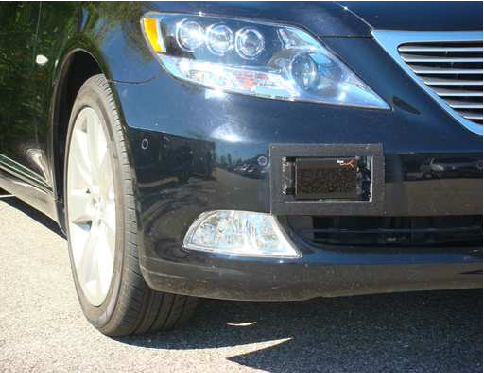
\includegraphics[width=0.40\columnwidth]{img/testbed:ibeo}
       &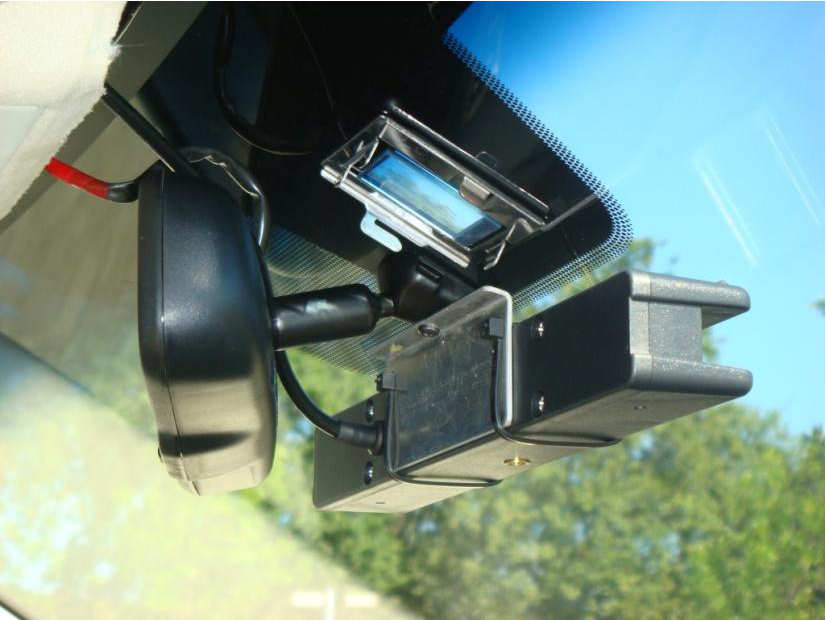
\includegraphics[width=0.40\columnwidth]{img/testbed:tyzx}
     \end{tabular}
   \caption{Lexus LS600h car equipped with two IBEO Lux lidars and a TYZX
     stereo camera}
   \label{fig:Lexus}
 \end{figure}

As the test platform requires a powerfull computer to process the stereo images in realtime, the car is equipped with a Dell workstation with an NVidia graphic card.

DeepSea TYZX stereo vision camera has a base line of 22 cm with 512x320 pixels of resolution and focal length of 410 pixels, this camera is provided with a library which can estimate the distance in cm of the objects captured by the camera, but in our tests we used the estimators developed at Inria\cite{PERROLLAZ-2010-493397}.
%better references
%http://ieeexplore.ieee.org/stamp/stamp.jsp?tp=&arnumber=6170895
%http://hal.inria.fr/index.php?halsid=fa9c2loot97ptftt2n38f6lvr5&view_this_doc=hal-00671208&version=1

\begin{figure}[h]
   \centering
     \begin{tabular}{lr}
       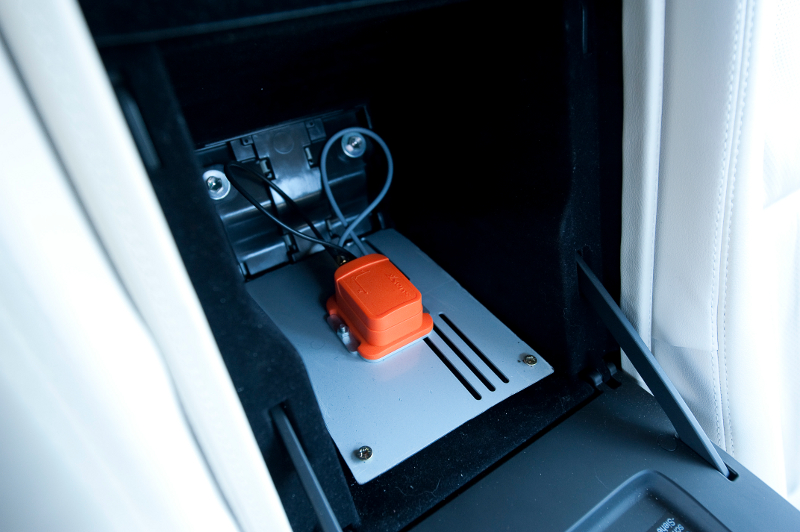
\includegraphics[width=0.45\columnwidth]{img/testbed:xsens}
       & 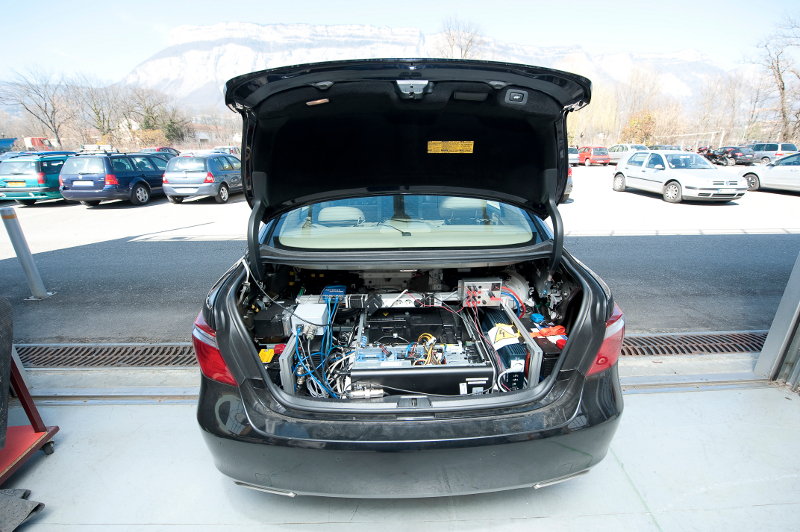
\includegraphics[width=0.45\columnwidth]{img/testbed:trunc}
     \end{tabular}
   \caption{MTi-G XSens IMU unit \& Intel Xeon 3.4GHz linux box}
   \label{fig:Lexus}
 \end{figure}

Each IBEO Lux Lidar is composed of four layers, each of them providing about 200 beams. The angular range of 100 degrees with angular resolution of 0.5 degrees. Each beam can reach until 200 m of distance measurement, with width of 40 m and maximum height of 2 m.

MTi-G XSens minimum of 120Hz and maximum of 512Hz for data logging and angular resolution of 0.05 degrees, all specifications are valid when considering an homogenous eletromagnetic environment. Maximum altitude operation is 18 Km and maximum speed is 515 m/s.



\subsubsection*{Software}

The high end cars are composed of several internal networks, each of them responsible to handle the transmission of the informations that are captured in that network to other one which need to process that information. This type of network is known as Controller Area Network (CAN) and provides a cheap and reliable way to communicate with devices, so CAN bus have been replacing the regular point-to-point wiring interconnection among the components\cite{bosch91can}.

Car manufacturers use platforms like YARP - Yet Another Robot Platform -, URBI or ROS to publish the information gathered by those networks, frameworks like ROS, allow the car to put the information into a shared memory array which can be access by other applications, the intent for most of those frameworks is to give longevity\cite{Fitzpatrick:2008:TLR:1327539.1327705} for the robot application that uses it by providing a platform that can evolve in cooperation manner with other projects.

For this project Robot Operating System(ROS) was adopted, ROS gives us the hability to save all information obtained during a run (driving the test platform) from all sensors, and replay it later in the laboratory, this by far allow to have a consistent test samples and a historical evolution of all scenarios gathered during the algorithm evolution, aloing the retro-performance benchmarking with other versions of the algorithm.

\subsubsection*{Assumptions}

\textit{Goal: What we assume to make our algorithm work}

\subsubsection*{Notation}

\paragraph{Occupancy Grid visual representation}

Representatiing the occupancy grid, implies in taking some precautions in the pattern used to represent each state, in this work the value $1$ represents occupied spaces and $0$ free spaces, although in the visual representation of the occupancy grid the $black$ dots represent occupied spaces and $white$ ones represent free spaces. In certain occasions, where the grid depicted is not binary, spaces where framework has absolutely no information about certain spaces (\textit{e.g.} due unreachability of the perception sensors in that sector), the color used is $gray$.

\subsection{Results}

\textit{Goal: What are our current results}

\subsection{Conclusion}

\textit{Goal: Express what we can conclude from this work, talk about future work, may be}
	
%=====================

\backmatter

\bibliographystyle{plain}
\bibliography{report}{}

\end{document}




